\chapter{\TitreChapitreUn}%
\label{chap:JetAtomique}

\bfigh
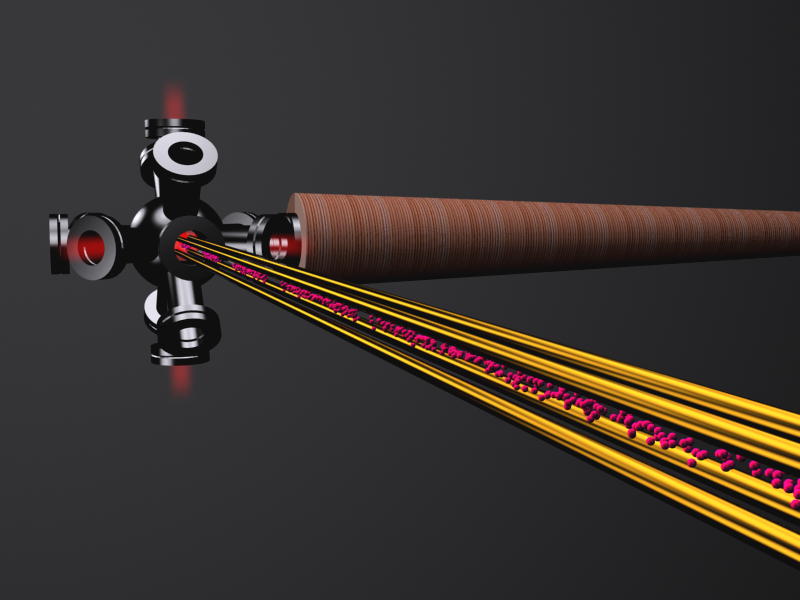
\includegraphics[width=\FigWidth]{P1/ChapitreJetAtomique}
\SansCaption
\efigh

\pagebreak

\minitoc
\vspace{0.5cm}

%Les deux premières parties de ce manuscrit auront pour objet l'étude du comportement d'ensembles atomiques se propageant dans un \gm. 
Ce chapitre a pour but d'introduire les concepts qui vont servir de support aux différentes analyses liées au guidage magnétique d'atomes. Nous y présenterons notamment le \setup tel qu'il était à mon arrivée dans l'équipe de \dgo. L'étude du \jatgm avait alors déjà montré que le \tcolel était suffisant pour pouvoir mettre en \oe uvre le \rpef. 
La plupart des thèmes abordés dans ce chapitre font l'objet d'une présentation détaillée dans la thèse de Thierry Lahaye~\cite{TTL} à laquelle il sera donc régulièrement fait référence.
Les concepts que j'ai eus à manipuler et les résultats importants obtenus lors de ma première année de thèse seront rappelés.

Dans ce chapitre, nous allons décrire la configuration magnétique choisie pour réaliser le guidage d'atomes sur notre \setup. Le principe d'obtention d'un jet \uf et intense d'atomes de \Rb sera ensuite détaillé. Nous aborderons la description du processus d'évaporation forcée, après avoir étudié les différentes manières de caractériser le jet.

\section{Piégeage dans un \gm \qp}\label{sec:PiegeageMagnetiqueGuide}

L'élément le plus caractéristique du \setup, qui a servi de support à ma première année de thèse, est un \gm d'une longueur $\Lguide=\m{4.5}$. 
Le guidage d'atomes neutres le long de structures filiformes parcourues par des courants est un domaine qui s'est fortement développé depuis une dizaine d'années~\cite{Sch95,KHR00,DLL00,TeR01,SBC01}. 
Cette section vise à décrire la configuration utilisée pour mener à bien le guidage d'un \jatuf et intense.

\casse

	\subsection{Configuration \qp de \chm}\label{sec:ConfigMagnetiqueGuide}
La configuration qui à été choisie sur notre \setup pour guider magnétiquement les atomes de \Rb est celle d'un \chm \qpdd~\cite{HiE00} créé par quatre tubes de cuivre parallèles parcourus par des courants deux à deux opposés (voir la figure~\nref{fig:TubesQuadrupole}).
%
\bfigh
\subfloat[Photo du \gm]{\label{TubesQuadrupole_0}
%\begin{overpic}
\includegraphics%
[height=6cm]{P1/TubesQuadrupole_0}
%\end{overpic}	
}\\
\subfloat[Lignes de champ]{\label{TubesQuadrupole_a}
%\begin{overpic}
\includegraphics%
[height=6cm]{P1/TubesQuadrupole_a}
%\end{overpic}	
}
\subfloat[Lignes équipotentielles]{\label{TubesQuadrupole_b}
%\begin{overpic}
\includegraphics%
[height=6cm]{P1/TubesQuadrupole_b}
%\end{overpic}	
}
\CaptionFig{Positionnement des tubes de cuivre et orientation des courants d'un système produisant un \chm \qpdd. \\
(a): Photographie représentant le \gm. Il est placé dans un tube de verre à l'intérieur duquel règne un vide poussé. On distingue l'une des pièces en céramique qui permet de maintenir les tubes de cuivre en position.\\
(b): Coupe dans le plan ($x,y$) perpendiculaire à l'axe du guide représentant le positionnement des tubes ainsi que quelques lignes de \chm. L'espacement entre deux tubes adjacents est noté $\espTubes$, et le courant qui les traverse est noté $I$. \\
(c): Schéma à l'échelle $3$ sur lequel sont représentées des équipotentielles (\cad des lignes suivant lesquelles le module du \chm est constant). Sur tout l'axe $z$, normal au plan de la figure, le module du champ s'annule. %Les lignes de champ représentées sur la figure (a) montrent bien une forte variation de la direction du vecteur champ autour du minimum.
}
\label{fig:TubesQuadrupole}
\efigh


L'expression du \chm créé par un tel système au voisinage de l'axe $z$ est:
\begin{equation}
	\vectBxyz = \vVecteur{-\gradB\,x}{\gradB\,y}{0} \mbox{\qquad avec \qquad} \gradB \equiv \frac{4\,\mu_0}{\pi\,\espTubes^2}\,I ,
	\label{eq:BQuadr}
\end{equation}
où $\gradB$ 
%
\nome{\gradB}{Gradient transverse de \chm au voisinage de l'axe $z$}
%
 est le gradient transverse de \chm au voisinage de l'axe $z$ et $\espTubes$ est l'espacement entre les axes de deux tubes adjacents
%
\nome{\espTubes}{Espacement entre les axes de tubes adjacents du \gm}%
. 
Cette expression est le résultat d'un développement limité à l'ordre~1 en $x$ et $y$ de la somme des contributions des \chms produits par les 4 tubes%
\footnote{L'utilisation de cette expression approchée conduit à faire une erreur inférieure à $\val{0.5}\%$ sur le module du \chm pour une distance à  l'axe typique de $\ttfrac{\espTubes}{4}$. C'est donc une très bonne aprroximation.}%
.

\ApplicationNumeriqueTitre{\gtchm}{
Calculons le gradient $\gradB$ sachant que:
\begin{itemize}
	\item le courant $I$ dans les tubes de cuivre du \gm peut monter jusqu'à une valeur de \SI{400}{\ampere},
	\item l'espacement entre deux tubes adjacents est $\espTubes=\mm{8}$.
\end{itemize}
En utilisant le courant maximal, on obtient un \gtchm :
\[
 \gradB = \SI{1}{\kilo G \per\centi\meter}
 \pointformule
\]
Pour comparaison, cette valeur est près de \val{10} fois supérieure à celles obtenues typiquement dans des pièges de \IP pour les expériences de \condbe. 
}
\Remarque{
La puissance dissipée par effet joule dans le guide peut atteindre quelques kilowatts. C'est pourquoi nous utilisons un système de refroidissement à eau. Celle-ci circule dans les tubes. On se reportera à la thèse de T.~Lahaye~\cite{TTL} pour avoir des détails sur les contraintes techniques liées à la mise en \oe uvre de ce \gm dans un environnement \uv.
}

\subsubsection{Piégeage magnéto-statique}
Dans les conditions de nos expériences, le potentiel magnétique d'un atome de \Rb immergé dans un champ $\Vecteur{B}$ est~\cite{MPP85}:
\begin{equation}
	U \approx \mF\,g_F\,\muB\,\modB ,
	\label{eq:EZeeman}
\end{equation}
où $\muB$ est le \termetech{magnéton de Bohr}, $g_F \approx \tfrac{(-1)^F}{2}$
est le facteur de Landé de l'état hyperfin de moment angulaire $F$ %
%\footnote{$\Module{g_F} = \tfrac{1}{4}\,(g_I + g_S)$ n'est pas tout à fait égal $\tfrac{1}{2}$, mais sa valeur en est proche à moins de $\val{E-3}$ près. On utilise généralement cette valeur, de la même manière qu'on utilise la valeur  $2$ pour le facteur gyromagnétique de l'électron.}%
 et $\mF$ est le nombre quantique magnétique de l'atome.
Dans toute la suite, nous aurons pour convention de noter :%
\nome{\mu}{Moment magnétique de l'atome}%
\[ 
\mu \equiv \mF\,g_F\,\muB
\virguleformule
\]
le moment magnétique de l'atome dans l'état $\Etat{F,\mF}$ considéré. Pour un atome de \Rb dans l'état $\EtatSFmF{1}{-1}$, on a $\mu\approx\SI{4.64}{\joule\per\tesla}$.
%La force qui dérive du potentiel~\nref{eq:EZeeman} 

\casse

\subsubsection{Confinement linéaire}
\inlinefig
{
\begin{tikzpicture}
\tkzInit[xmin=-3,xmax=3,ymin=-0,ymax=4]
\tkzX[ orig, noticks,label=$r$]%,poslabel=-0.5cm]
\tkzY[label=$\Ulin$, noticks]
\tkzFct[samples = 200,lw = 1pt,color = red](-4..4){(2*x*x+0)**(0.5)}
%\tkzFct[samples = 200,lw = 1pt,color = gray, style=dashed](-4..4){(2*x*x+0)**(0.5)}
\end{tikzpicture}
}
Pour la configuration décrite ci-dessus, le potentiel auquel sont soumis les atomes dans le \gm est:
\begin{align}
	\Ulin(x,y,z) 	&= \mu\,\sqrt{\Bx^2+\By^2+\Bz^2} \nonumber \\
	       				&= \mu\,\gradB\,\sqrt{x^2+y^2} ,\nonumber 
	\label{eq:PotentielTubesLinXY}
\end{align}
que nous pouvons aussi mettre sous la forme:
\begin{equation}
	\Ulin(r) = \mu\,\gradB\,r
	\label{eq:PotentielTubesLin}
\end{equation}
\picskip{0}
\noindent où $r \equiv \sqrt{x^2+y^2}$ sera la distance à l'axe $z$. 
\nome{r}{Distance à l'axe du \gm}%
Ce potentiel sera qualifié de \emph{linéaire}. 


\subsubsection{Confinement hyperbolique}
%Comme nous l'avons mentionné dans la section~\nref{sec:PiegeageMagnetique}, le phénomène de pertes par retournement de spin est présent dans les zones de faible \chm. Or 
Vis-à-vis du piégeage magnéto-statistique d'atomes \ufs, le principal défaut du confinement linéaire dont il est question ci-dessus est de voir son champ s'annuler sur tout l'axe $z$. 
On peut alors voir apparaître un phénomène de pertes par retournement de spin (ou pertes Majorana~\cite{SuB97}).
Il est cependant possible de s'affranchir de ce défaut en superposant un \chm uniforme $\vectB = \Bpara\,\Vecteur{e_z}$ %
\nome{\Bpara}{Champ magnétique uniforme selon l'axe de guide}%
suivant l'axe $z$ du \gm. Ce champ est qualifié de \emph{longitudinal}.

\inlinefig
{
\begin{tikzpicture}
\tkzInit[xmin=-3,xmax=3,ymin=-0,ymax=4]
\tkzText(1.4,0.8){$\mu\,\Bpara$}
\tkzHLine[style=dotted]{1}
\tkzX[label=$r$, orig, noticks]%, poslabel=-.5cm]
\tkzY[label=$\Uhyp$, noticks]
\tkzFct[samples = 200,lw = 1pt,color = red](-4..4){(2*x*x+1)**(0.5)}
\tkzFct[samples = 200,lw = 1pt,color = gray, style=dashed](-4..4){(2*x*x+0)**(0.5)}
\end{tikzpicture}
}
\noindent L'expression du potentiel devient alors:
\begin{align}
	\Uhyp(x,y,z) 	&= \mu\,\sqrt{\Bx^2+\By^2+\Bz^2} \nonumber \\
								&= \mu\,\sqrt{\gradB^2\,\left( x^2 + y^2 \right) + \Bpara^2} ,\nonumber 
	\label{eq:PotentielTubesHypXY}
\end{align}
que nous pouvons aussi mettre sous la forme:
\begin{equation}
	\Uhyp(r) = \mu\,\sqrt{\gradB^2\,r^2 + \Bpara^2}
	\virguleformule
	\label{eq:PotentielTubesHyp}
\end{equation}
\picskip{1}\noindent qui est de forme hyperbolique et présente l'avantage de n'avoir aucune zone de \chm nul puisque celui-ci prend pour valeur minimale $\Bpara$ sur l'axe $z$. 

En contrepartie, le potentiel est moins confinant que dans le cas linéaire. 
Mathématiquement, l'expression de la force de rappel radiale
%, $- \ttDerive{\Uhyp(r)}{r}$ 
peut se mettre sous la forme :
\[ 
F(r) \equiv - \Derive{\Uhyp(r)}{r}=-\mu\,\gradB\,\frac{1}{\sqrt{ 1 + \frac{\Bpara^2}{\gradB^2\,r^2 } }}
\virguleformule
 \]
qui est clairement moins intense (à cause du dénominateur strictement supérieur à $1$) que dans le cas linéaire ($ - \tDerive{\Ulin(r)}{r} = -\mu\,\gradB$) et 
tend même vers $0$ au voisinage de l'axe $z$. 


\ApplicationNumeriqueTitre{Quelle valeur prendre pour $\Bpara$ ?}{
\label{AN:ValeurB0}
La superposition d'un \chm longitudinal à pour effet secondaire indésirable de rendre le potentiel moins confinant.
Nous devons donc utiliser une valeur de $\Bpara$ la plus petite possible, mais qui soit compatible avec de faibles pertes par retournement de spin, à savoir que
%\cad D'après la remarque page \pageref{Rq:Majorana}, 
les variations du \chm \sotosay{vu} par les atomes le long de leurs trajectoires doivent rester lentes devant l'échelle de temps définie par la précession de Larmor. Or:
\begin{itemize}
	\item nous verrons dans la suite que la pulsations d'oscillation $\omega$ est de l'ordre du $\SI{}{\kilo\hertz}$. Celle-ci donne l'ordre de grandeur des taux de variation du champ \sotosay{vu} par un atome.%: $\tfrac{\left| \mathrm{d} \vectB}{\mathrm{d}t} \right| \approx \left| \right|$
	\item la fréquence de Larmor $\omegaL$ est d'environ $\SI{1}{\mega\hertz\per G}$
\end{itemize} 
Afin d'assurer l'inégalité $\omegaL \gg \omega$, un champ $\Bpara$ de quelques centièmes de Gauss est suffisant. Cependant, on ne peut pas utiliser de si faibles valeurs car l'environnement du laboratoire est pollué par des ondes radio basses fréquences qui pourraient induire des pertes par retournement de spin~\cite{ViG96}. En pratique, nous utilisons typiquement :
$
\Bpara = \SI{0.5}{G}
\pointformule
$
%\finformule
}

%\Remarque
{
%\label{Rq:alpha}
\subsubsection{Comportement asymptotique du potentiel hyperbolique}
La superposition du champ longitudinal $\Bpara$ a pour conséquence de \sotosay{déformer} le potentiel linéaire $\Ulin(r)$ dont il est question plus haut. 
Cette déformation intervient en fait de manière notable dans les zones de faible \chm ($\modB \lesssim \Bpara$). Ceci nous permet de définir une distance à l'axe caractéristique $\Rdef$, au delà de laquelle le potentiel linéaire est peu déformé:%
%\nome{\Rdef}{Distance ty}
\[
 \Rdef \equiv \frac{\Bpara}{\gradB}
 \pointformule 
 \]
Ainsi, si nous considérons le potentiel hyperbolique $\Uhyp(r)$ pour des distances à l'axe $r \gg \Rdef$, celui-ci est \emph{comme le potentiel linéaire}. D'après l'expression~\nref{eq:PotentielTubesLin}, cette distance $\Rdef$ définit une énergie $\Udef$:%
\nome{\Udef}{Potentiel magnétique sur l'axe du guide}%
\[
 \Udef \equiv \mu\,\gradB\,\Rdef = \mu\,\Bpara
 \virguleformule
\]
qui correspond à une plage caractéristique d'énergie sur laquelle le potentiel linéaire a été notablement déformé. Donc, si les atomes du jet possèdent une énergie \thiq $\kb\,T$ suffisante (grande devant $\Udef$), ils vont explorer une plage de distances $r \gg \Rdef$ et le potentiel \sotosay{vu} par les atomes sera essentiellement linéaire.
}

\Resultat
{
\label{Rq:alpha}
Ainsi, il sera utile pour la suite de considérer le paramètre sans dimension $\alpha$ défini par:
\begin{equation}
	\alpha \equiv \frac{\Udef}{\kb\,T} =  \alphaexpr 
	\pointformule
	\label{eq:alpha}
\end{equation}
\finformule
}%
\nomeRemonte{\alpha}{Paramètre sans dimension caractérisant le confinement \sotosay{vu} par les atomes}{1.7cm}%

\casse

\noindent Le paramètre $\alpha$ caractérise, comme on le voit sur la figure~\nref{fig:alpha}, le confinement tel qu'il est \sotosay{vu} par les atomes:
\begin{itemize}
	\item si $\alpha \ll 1$, cela signifie que les atomes ont assez d'énergie \thiq pour explorer essentiellement la plage linéaire du potentiel%
%\footnote{Si l'on considère le potentiel comme étant linéaire, un rapide calcul montre que la proportion d'atome ayant une distance à l'axe inférieure à $\Rdef$ est .}%
. 
On pourra donc considérer que: \[ \Uhyp(r) \approx \mu\,\gradB\,r \]
	\item si $\alpha \gg 1$, les atomes n'explorent que le fond du potentiel hyperbolique, dans une zone sur laquelle nous pouvons effectuer un développement limité de $\Uhyp(r)$ autour de $r=0$. On pourra donc considérer que: 
\[ 
\Uhyp(r) \approx \frac{1}{2} \, m \, \omega^2\,r^2 + \const, \mbox{\qquad avec \qquad} \omega = \sqrt{\frac{\mu\,\gradB^2}{m\,\Bpara}} 
= \frac{\mu\,\gradB}{\sqrt{\alpha\,m\,\kb\,T}}
\pointformule
\]
\end{itemize}  

%\AjouteLigne
%\AjouteLigne

%
\bfighs
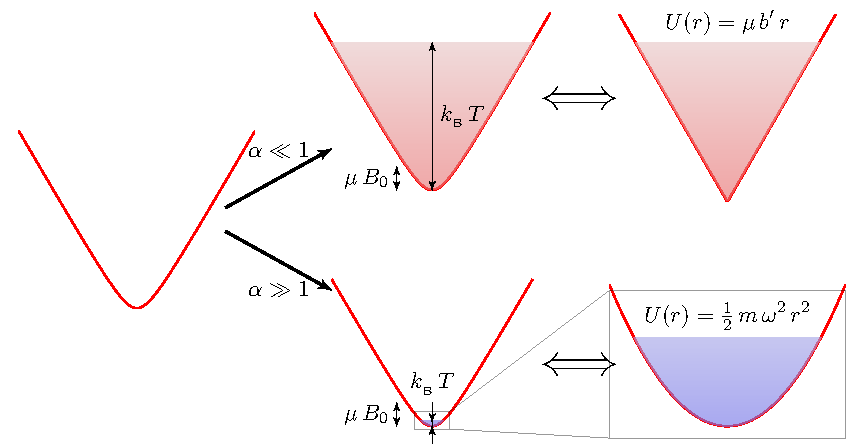
\includegraphics{P1/alpha}
\CaptionFigssss{Représentation schématique du \ppt. Si la température du \jat est élevée (\ie: $\kb\,T \gg \mu\,\Bpara$), le potentiel hyperbolique peut être considéré comme étant essentiellement linéaire. Si à l'inverse sa température est faible (\ie: $\kb\,T \ll \mu\,\Bpara$), les atomes explorent essentiellement le fond du potentiel, que l'on peut alors considérer comme étant harmonique.
}
\label{fig:alpha}
\efigh

%\AjouteLigne

\ApplicationNumerique
{Pour des conditions typiques de notre expérience, le \jat possède une température d'environ \microK{600}. Pour une valeur de champ longitudinal $\Bpara=\gauss{0.5}$, nous calculons le paramètre $\alpha \approx \val{0.025}$. Ceci traduit le fait que le jet est soumis à un \ppt essentiellement linéaire.
L'extension transverse du jet dans le guide correspond typiquement à :
\RemonteUnPeuFig
\[
R \approx \frac{\kb\,T}{\mu\,\gradB} \approx \mm{0.25}
\pointformule
\RemonteUnPeuFig
\]
Dans un tel potentiel linéaire, la période d'oscillation radiale d'un atome dépend de sa trajectoire, mais est typiquement de l'ordre de :
\RemonteUnPeuFig
\[
\tau \approx \sqrt{\frac{2\,R\,m}{\mu\,\gradB}} \approx \ms{1}
\pointformule
\]
\finformule
}

\casse

	\subsection{Guidage \ma d'un \jatuf}\label{sec:GuidageJet}
	Dans la sous-section précédente nous avons décrit le potentiel $\Uhyp(r)$ auquel sont soumis les atomes de \Rb dans le \gm. Nous voulons maintenant discuter des caractéristiques d'un \jat s'y propageant. Pour ce faire, nous allons considérer ici un \j à l'\eqthdy confiné radialement par le potentiel $\Uhyp(r)$. De plus, nous ne considèrerons que le cas d'un jet supersonique dont la vitesse moyenne $\vjet$ %
\nome{\vjet}{Vitesse moyenne du jet se propageant selon l'axe $z$ du \gm}%
est \emph{plusieurs fois supérieure} à sa \dispvitlong $\deltavjet$. De cette manière, on s'assure que tous les atomes possèdent une vitesse $\vz > 0$ %
%\nome{\vz}{Vitesse d'un atome selon l'axe $z$ du \gm}%
	suivant l'axe $z$ du \gm (on parle alors d'un jet \emph{monocinétique} suivant l'axe $z$). En pratique, nous choisissons d'avoir:
$
	\vjet \geq 3\,\deltavjet
	\pointformule
$
	\subsubsection{Paramètres décrivant le \jat}
En considérant le problème comme étant invariant par translation suivant l'axe $z$, les seuls paramètres qui décrivent le \jat confiné dans le potentiel hyperbolique $\Uhyp(r)$ sont:
%\Resultat{
%\paragraph{les paramètres du jet:}
	\begin{itemizel}
	\item la vitesse moyenne $\vjet$ du jet
	\item son \fat $\flux$,%
\nome{\flux}{Flux atomique du jet}%
	\item sa température $T$ d'équilibre dans le référentiel en mouvement à la vitesse $\vjet$,
%\end{itemize}
%\paragraph{et les paramètres du confinement transverse:}
%	\begin{itemize}
	\item le gradient transverse $\gradB$ de \chm,
	\item le champ longitudinal $\Bpara$, ou de manière équivalente, le paramètre $\alpha$ qui donne la forme du potentiel hyperbolique pour une température donnée.
\end{itemizel}
%}
%
Ces 5 paramètres $(\vjet, \flux, T, \gradB, \alpha)$, relatifs à un jet à l'\eqthdy, permettent d'exprimer toutes les autres grandeurs physiques importantes qui doivent être prises en compte pour l'étude du refroidissement par évaporation:
%\Resultat{
\begin{itemizel}
	\item la \dat $\njet(r)$ du jet. Sa valeur maximale, sur l'axe $z$ du guide, est notée $\njetaxe$, %
\nome{\njet(r),\njetaxe}{Densité atomique du jet, et sa valeur maximale, sur l'axe $z$ du guide}%
	\item la \ddedpup $\rho(r)$ dont la valeur sur l'axe du guide est noté $\rhojetaxe$, %
\nome{\rho(r),\rhojetaxe}{Densité dans l'\edp, et sa valeur maximale, sur l'axe $z$ du guide}% 
	\item le \tcolel moyen par atome $\gammacol$ au sein du jet, %
\nome{\gammacol}{Taux moyen de \colel par atome au sein du jet}%
	\item le \Ncolel moyen par atome $\Ncol$ tout au long de la propagation dans le \gm, %
\nome{\Ncol}{Nombre moyen de \colel par atome au sein du jet}%
	\item l'énergie mécanique moyenne $\Emoy$ d'un atome du jet. %
\nome{\Emoy}{Énergie mécanique moyenne par atome au sein du jet}%
\end{itemizel}
%}
\EnFaitNon{
La \fdddedpup à l'\eqthdy est donnée par la distribution de Boltzmann:
\[	\fjet(x,y,v_x,v_y,v_z) = C\,\Expo{-\frac{\Ham}{\kb\,T}} ,\]
où $\Ham$ désigne l'hamiltonien d'une particule qui s'exprime notamment grâce à la relation \vref{eq:PotentielTubesHyp}. Le facteur de normalisation $C$ sera choisi de manière à assurer que l'intégrale de $\fjet$ donne la \datlin suivant l'axe $z$ du guide. Nous pouvons donc écrire $\fjet$ sous cette forme:
\begin{align}
	\fjet(r,\vtrans, v_z)
	& = \frac{\flux}{\vjet} \, \fjetTrans(r, \vtrans) \, \fjetPara(\vz) \\
	\mbox{avec \quad} 
	& \fjetTrans(r, \vtrans)
	=  \Expo{-\frac{\mu\,\sqrt{\gradB^2\,r^2 + \Bpara^2}}{\kb\,T}} 
	 \, \Expo{-\frac{m\,\vtrans^2}{2\,\kb\,T}} \nonumber \\
  \mbox{et \quad} 
	& \fjetPara(\vz)
  = \Expo{-\frac{m\,\left(\vz-\vjet\right)^2}{2\,\kb\,T}}\nonumber 
	\label{eq:FjetBoltzmann}
\end{align}
MONOCINETIQUE ! ! ! 
}
\noindent Nous donnons ici l'expression de chacune de ces grandeurs~\cite{TTL}: 
\begin{subequations}
\begin{align}
	\njetaxe & = \frac{1}{2\,\pi}\,\frac{1}{1+\alpha}\,\frac{\flux}{\vjet}\,\left( \frac{\mu\,\gradB}{\kb\,T} \right)^2 
	\virguleformule 
	\label{eq:njetaxe}
	\\
	\rhojetaxe & \equiv \njetaxe \, \lambdaDB^3 = \frac{1}{2\,\pi}\,\frac{1}{1+\alpha}\,\frac{\flux}{\vjet}\,\left( \frac{\mu\,\gradB}{\kb\,T} \right)^2
	\,\, \frac{h^3}{(2\,\pi\,m\,\kb\,T)^{3/2}} 
	\virguleformule 
	\label{eq:rhojetaxe}
	\\
	\gammacol & = \frac{\sigma}{2\,\pi^{3/2}} \, \frac{1+2\,\alpha}{(1+\alpha)^2} 
	\, \frac{\flux}{\vjet} \, \left( \frac{\mu\,\gradB}{\kb\,T} \right)^2 
	\, \sqrt{\frac{\kb\,T}{m}} 
	\virguleformule 
	\label{eq:gammacol}
	\\
	\Ncol & \equiv \gammacol \, \frac{\Lguide}{\vjet} =
	\frac{\sigma}{2\,\pi^{3/2}} \, \frac{1+2\,\alpha}{(1+\alpha)^2} 
	\, \frac{\flux\,\Lguide}{\vjet^2} \, \left( \frac{\mu\,\gradB}{\kb\,T} \right)^2 
	\, \sqrt{\frac{\kb\,T}{m}} 
	\virguleformule 
	\label{eq:Ncol}
	\\
 	\Emoy & = \kb\,T\,\frac{2+\alpha}{1+\alpha} 
	\pointformule
	\label{eq:Emoy} 
\end{align}
\end{subequations}
Dans l'expression~\nref{eq:Emoy}, l'énergie potentielle est prise comme étant nulle au fond du piège (en $r=0$) et $\sigma$ %
\nome{\sigma}{Section efficace de collision dans l'onde $s$}%
est la section efficace de collision dans l'onde $s$ (supposée indépendante de l'énergie cinétique des atomes).


\casse


Notons que les lois d'échelles pour un confinement donné permettent de mieux comprendre l'évolution des propriétés du \jatg en fonction des paramètres $(\vjet, \flux, T)$ que nous pouvons faire varier dynamiquement (voir la section \vref{sec:EvapRf}). 
\Resultat
{
Nous envisageons les deux cas limites:  $\alpha \ll 1$ (le potentiel ressenti par les atomes est essentiellement linéaire) et $\alpha \gg 1$ (le potentiel ressenti par les atomes est essentiellement harmonique):
\newcommand{\grostruc}{\vphantom{$
{\dfrac{\flux^{{\vjet\,T^{\frac{3}{2}}}}
}{\vjet\,T^{\frac{3}{2}}_{{\vjet\,T^{{3}{2}}}}
}}$}}
\label{RQ:ProportionProprieteJet}
\begin{center}
\begin{large}
\begin{tabular}{rcc|cc}
\vphantom{${{{{{{{{{A^A}_A}_A}_A}_A}_A}_A}_A}_A}$} \qquad &  \qquad\qquad   
&  $\qquad \alpha \ll 1 \qquad$ & $ \qquad \alpha \gg 1 \qquad$ 
&\\
\cline{3-4}
\grostruc   $\njetaxe $& $\propto$   & $ \frac{\flux}{\vjet\,T^2} $ & $  \frac{\flux}{\vjet\,T} $ 
&\\
\cline{3-4}
\grostruc   $\rhojetaxe $ & $\propto$ & $ \frac{\flux}{\vjet\,T^{\frac{7}{2}}} $ & $  \frac{\flux}{\vjet\,T^{\frac{5}{2}}} $ 
&\\
\cline{3-4}
\grostruc   $\gammacol $ & $\propto$  & $ \frac{\flux}{\vjet\,T^{\frac{3}{2}}} $ & $  \frac{\flux}{\vjet\,\sqrt{T}} $ 
&\\
\cline{3-4}
\grostruc   $\Ncol $ & $\propto$  & $ \frac{\flux}{\vjet^2\,T^{\frac{3}{2}}} $ & $  \frac{\flux}{\vjet^2\,\sqrt{T}} $ 
&\\
\cline{3-4}
$\vphantom{T^{{\vjet\,T^{\frac{3}{2}}}}}$   $\Emoy $ & $=          $  & $ 2\,\kb\,T $ & $ \kb\,T $
&\\
\end{tabular}	
\end{large}
\end{center}
}
Il est donc clairement intéressant de disposer d'un \jat intense, \uf est lent.

%\Resultat
%{\label{RQ:ProportionProprieteJet}
%\begin{center}
%\begin{large}
%\begin{tabular}{lccc}
%                  &     & ~ \qquad $ \alpha \ll 1$ \qquad ~ & $ \alpha \gg 1 $ 
%   \vspace{1ex}
%\\
%   $\njetaxe $& $\propto$   & $ \frac{\flux}{\vjet\,T^2} $ & $  \frac{\flux}{\vjet\,T} $ 
%   \vspace{1ex}
%\\
%   $\rhojetaxe $ & $\propto$ & $ \frac{\flux}{\vjet\,T^{\frac{7}{2}}} $ & $  \frac{\flux}{\vjet\,T^{\frac{5}{2}}} $ 
%   \vspace{1ex}
%\\
%   $\gammacol $ & $\propto$  & $ \frac{\flux}{\vjet\,T^{\frac{3}{2}}} $ & $  \frac{\flux}{\vjet\,\sqrt{T}} $ 
%   \vspace{1ex}
%\\
%   $\Ncol $ & $\propto$  & $ \frac{\flux}{\vjet^2\,T^{\frac{3}{2}}} $ & $  \frac{\flux}{\vjet^2\,\sqrt{T}} $ 
%   \vspace{1ex}
%\\
%   $\Emoy $ & $=          $  & $ 2\,\kb\,T $ & $ \kb\,T $ \\
%\end{tabular}	
%\end{large}
%\end{center}
%}



\section{De l'injection pulsée de \pats à l'obtention d'un \j continu}\label{sec:FormationJetContinu}
Cette section présente la technique utilisée pour produire un \jatuf et intense dans le \gm. 

	\subsection{Pourquoi une injection pulsée?}
L'équipe de \dgo, dans laquelle j'ai effectué ma thèse, est la première à avoir réalisé le guidage d'un \jaf~\cite{CRA02}. Deux techniques expérimentales différentes ont été mises au point afin de produire ce jet en couplant les atomes d'un \pmo à un \gm:
\begin{itemizel}
	\item la première consiste à \emph{injecter en continu} les atomes. Pour ce faire, le piégeage magnéto-optique est réalisé uniquement suivant les deux directions transverses. Suivant l'axe du guide, les atomes \emph{fuient} vers l'entrée du guide grâce une technique de mélasse mouvante. Notons que, l'injection étant continue, il n'est pas possible d'optimiser simultanément la capture des atomes et leur lancement. 
	\item la deuxième repose sur \emph{l'injection pulsée de \pats}. La \dispvitlong des \pats se propageant dans le guide induit un étalement suivant l'axe du \gm. Le recouvrement de ces \ps permet ainsi la formation d'un \jat continu, après une distance de propagation de typiquement \cm{50}.
\end{itemizel} 


\casse


Ces deux méthodes d'injection donnaient alors des performances similaires en terme de flux ($\approx \atparsec{3E8}$) du \jat. En revanche, sa température était dix fois inférieure en utilisant la deuxième technique ($\approx \microK{100}$)~\cite{RCL03}. Cela est principalement dû à deux raisons:
	\begin{itemize}
	\item le contrôle dynamique des paramètres du \pmo permet de combiner un très bon taux de capture, suivi d'un refroidissement très efficace par une technique de mélasse optique.% (se reporter à la section \vref{sec:EtapesRefroidissement}).
	\item la présence en continu d'un \pmo détruit partiellement le \jgm du fait de la diffusion de lumière sur la transition \termetech{repompeur} (les atomes sont en effet préparés dans l'état $\EtatSFmF{1}{-1}$). L'injection pulsée permet quant à elle, après l'injection, de laisser chaque \p s'éloigner dans le guide avant de charger le \p suivant. Le \fat moyen observé est plus important%
	\footnote{Le \fat est, dans le cas de l'injection pulsée, une fonction croissante de la distance entre deux \pss: plus la distance qui sépare le \pmo du \p précédemment injecté est grande, moins la lumière \termetech{repompeur} affectera celui-ci.} quand on utilise une injection pulsée.
\end{itemize}

	\subsection{Formation de \pats ultra-froids}\label{sec:PaquetsPmo}
Nous rappelons ici brièvement les choix retenus pour une alimentation optimale du \pmo. 
%décrivons ici la manière dont les \pats sont obtenus. 
La figure~\nref{fig:VueEnsembleSetupJet} représente une vue d'ensemble du \setup. Les différents éléments qui le constituent sont détaillés dans le chapitre 2 de la thèse de T.~Lahaye~\cite{TTL}. 
Nous donnerons donc simplement les paramètres importants qui caractérisent les principales parties de notre \setup:
	\begin{itemize}
	\item \textbf{un four à recirculation%
	\footnote{La dénomination de \termetech{four} provient du fait qu'un échantillons de rubidium solide est chauffé (à typiquement \val{100}-\SI{150}{\degreecelsius}), et ce afin d'augmenter sa pression de vapeur saturante. Le four est ainsi empli d'une vapeur de rubidium, qui s'échappe dans le système à \uv pour alimenter le \pmo. La dénomination de \termetech{four à recirculation} provient du fait que la géométrie du four permet de récupérer automatiquement une partie du rubidium inutilisé. Ceci permet d'augmenter considérablement la durée d'utilisation du four~\cite{TTL}.}%
} dont la conception est inspirée de la référence~\cite{CaP78} fournit un jet collimaté d'atomes de \Rb avec un flux d'environ $\atparsec{2E12}$ et une vitesse moyenne de l'ordre de \mps{400}.
	\item \textbf{un \ZS}\cite{PhM82,PPM82,PMP85} d'un mètre de long ralentit $10\%$ des atomes provenant du four à une vitesse moyenne de l'ordre de \mps{20}. Le flux obtenu, d'environ $\atparsec{2E{11}}$, fait de ce \ZS l'un des plus performants au monde.
	\item \textbf{un \pmo de géométrie allongée} capture une partie des atomes ralentis par le \ZS. Le taux de capture est d'environ $\atparsec{2E10}$. Le nombre d'atomes sature rapidement ($\approx\seconde{1}$) à environ $\val{E10}$ atomes. Notons que ce taux de chargement est nettement supérieur à ceux observés dans les expériences typiques de \condbe.
\end{itemize}
%
\bfigh
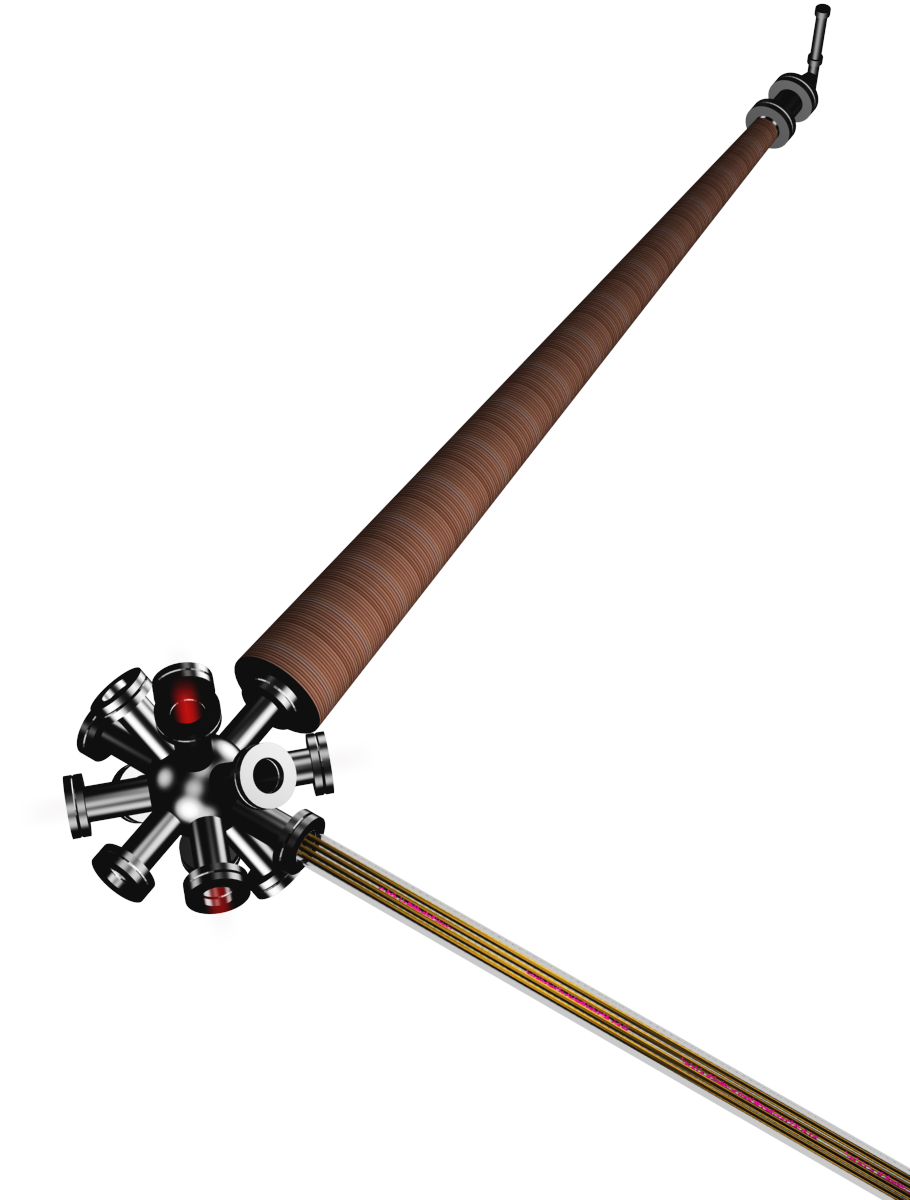
\includegraphics{P1/VueEnsembleSetupJet}
\CaptionFig{Schéma représentant une vue d'ensemble du \setup. 
}
\label{fig:VueEnsembleSetupJet}
\efigh
%
\Resultat{
Grâce à ce \setup, il nous est ainsi possible de produire un \pat contenant typiquement  $\Npat = \val{2E9}$ atomes en $\ms{100}$.
}
La température d'un tel \pat capturé dans le \pmo dépend de plusieurs facteurs (désaccord des lasers, nombre d'atomes, gradient de \chm,...), mais ce situe typiquement dans la plage \val{100}-\microK{200}. Une phase de mélasse optique permet d'obtenir une température d'environ \val{20}-\microK{30}.


\casse


	\subsection{Technique d'injection dans le \gm}\label{sec:InjectionGuide}
	Le couplage des atomes du \pmo dans le \gm est une étape délicate. De manière à mettre en mouvement le \pat, nous utilisons une technique de \emph{mélasse mouvante}%, qui fut initialement développée dans le contexte des horloges atomiques à fontaine d'atome froids 
~\cite{CSG91}. La mise en \oe uvre de cette technique dans le \setup, ainsi que les détails relatifs au pompage optique des atomes dans l'état piégé \EtatFmF{1}{-1} et au guidage des \ps vers l'entrée du \gm, sont détaillés dans la thèse de T.~Lahaye~\cite{TTL}.
Nous nous contenterons ici de mentionner les quatre étapes de notre \seqexp qui est répétée environ 5 fois par seconde:
\begin{enumerate}
	\item Capture dans le \pmo pendant \ms{100} d'atomes issus du \ZS : les lasers du \pmo sont désaccordés de $\delta=-3\,\Gamma$ et les gradients de \chm valent typiquement \gausspcm{5} transversalement et \gausspcm{0.5} selon l'axe longitudinal.
	\item \termetech{Mélasse optique mouvante} de \ms{3}. Le désaccord des lasers est alors:
	\begin{itemize}
		\item gardé constant à $\delta=-3\,\Gamma$ pendant \ms{1.5},
		\item puis augmenté linéairement jusqu'à $\delta=-12\,\Gamma$ en \ms{1.5}.
	\end{itemize}
	\item \termetech{Pompage optique} (pendant \ms{0.7}) dans le \snZ $\EtatSFmF{1}{-1}$.
	\item \termetech{Pré-guidage \ma} du \pat pendant environ \ms{100}. Cette phase consiste à prévenir l'expansion transverse ainsi que la chute libre du \p avant son arrivée dans le guide dont l'entrée est située à \cm{5} du \pmo. En pratique, un \gtchm d'environ \gausspcm{100} est produit par les bobines du \pmo.
\end{enumerate}
%
\Resultat{
L'optimisation de cette procédure lors de la première année de ma thèse a permis de produire un \jatg dont les caractéristiques $(\vjet, \flux, T)$ sont:
\begin{itemize}
	\item $\vjet = \cmps{60}$ (voir la remarque \vpageref[ci-dessous]{Rq:InjectionPente}),
	\item $\flux = \atparsec{7E9}$,
	\item $T = \microK{600}$.
\end{itemize}
}
Ces paramètres sont obtenus pour un confinement caractérisé par un \gtchm $\gradB = \gausspcm{800}$ et un champ longitudinal $\Bpara = \gauss{0.5}$. Le paramètre $\alpha=\ttfrac{\mu\,\Bpara}{\kb\,T}$ vaut dans ces conditions $\alpha = \val{0.025}$, traduisant le fait que le jet est soumis à un \ppt essentiellement linéaire (voir la \autoref{sec:ConfigMagnetiqueGuide}).
%
\ApplicationNumerique{
Calculons, grâce aux expressions \vrefrange{eq:njetaxe}{eq:gammacol}, les autres caractéristiques du jet pour les valeurs énoncées ci-dessus:
\begin{itemize}
	\item \dat sur l'axe $z$: $\njetaxe = \atpcc{3.6E10}$,%3,6125
	\item \ddedpup sur l'axe $z$: $\rhojetaxe = \val{1.7E{-8}}$,%1,694
	\item $\gammacol = \val{3.6}$ collisions par seconde et par atome.%3,580
	\item $\Ncol \approx 20$ collisions tout au long de la propagation dans le \gm.
\end{itemize}
}

\casse


\subsubsection{Utilisation d'une \secpent pour ralentir le jet}
{\label{Rq:InjectionPente}
Notons que la vitesse d'injection des \pats est $\vinj = \cmps{90}$. La vitesse du jet $\vjet = \cmps{60}$ est obtenue par la mise en place d'une \secpent, ayant un dénivelé de \mm{22} sur les premiers \m{1.7} du \gm (voir la figure \vref{fig:Montage10Antennes}).
On peut se demander quel est l'avantage à effectuer cette procédure de ralentissement sachant qu'il est techniquement possible de communiquer une vitesse initiale $\vinj = \cmps{60}$ aux \ps. 

La raison en est, comme nous l'avons évoqué précédemment, que le \fat est d'autant plus élevé que la distance qui sépare le \pmo du \p précédemment injecté est grande (à cause de la lumière repompeur diffusée par le \pmo). Le fait d'injecter les \ps à une vitesse relativement élevée permet d'augmenter cette distance (pour un taux de répétition donné), et donc d'augmenter le \fat. 

En revanche, les expressions \vrefrange{eq:njetaxe}{eq:gammacol}, montrent que nous avons tout intérêt à disposer d'un jet le plus lent possible. La procédure de ralentissement est donc un moyen de combiner un flux élevé à une vitesse faible. 
}


\subsection{Entrée non-adiabatique du jet dans le \gm}\label{sec:EntreeGuideNonAdiabatique}

Étant donnée la température du \nat durant la phase de mélasse optique (soit typiquement \val{20}-\microK{50}), on peut se demander pourquoi le jet possède une température si élevée (\microK{600}). Ceci est dû au fait que chaque nuage, subit une \emph{compression transverse} non-adiabatique lors de l'allumage du pré-guide, ainsi qu'à l'entrée du \gm. L'énergie fournie au nuage est d'autant plus élevée que son extension transverse est grande\footnotemark. 
%Nous verrons d'ailleurs dans le chapitre~\nref{chap:MiroirMobile}, que la \dispvitlong d'un \p individuel dans le \gm n'est que de 
\footnotetext{Plus l'extension transverse du nuage est faible, moins il sera sensible à une augmentation de la force de confinement. D'ailleurs, si on imagine un ensemble d'atomes réunis sur l'axe $z$ du \gm, ceux-ci se propageant selon une ligne de \chm nul seront insensible à l'augmentation du \gtchm.}
\ApplicationNumerique
{
On peut estimer l'ordre de grandeur de l'échauffement en considérant l'extension transverse d'un nuage, $2\,r\approx\mm{1}$ et le \gtchm du guide, $\gradB \approx \gausspcm{800}$. Lors de l'entrée non-adiabatique des atomes dans le guide, ceux-ci vont se voir fournir une énergie potentielle moyenne de l'ordre de:~$\mu\,\gradB\,r$, qui correspond à $\kb\times\milliK{2}$.
Les collisions entre atomes vont cependant conduire à une redistribution de l'énergie sur les autres degrés de libertés et la température d'équilibre du jet n'augmentera finalement que de typiquement\footnotemark~\milliK{1}.
}
\footnotetext{La fraction d'énergie qui se répartit sur chaque degrés de liberté des atomes fait intervenir le théorème du viriel et est exposé dans la remarque \vpageref{Rq:Viriel}.}

\ifthenelse{\FormatEUE > 0}{}
{\AjouteLigne}
\RemonteUnPeuFig\RemonteUnPeuFig\RemonteUnPeuFig
\subsubsection{Température longitudinale des \ps individuels}
Dans le chapitre~\nref{chap:MiroirMobile}, nous serons amenés à considérer la propagation libre de \pats individuels dans le \gm. Nous y montrerons que, par une technique de \termetech{temps de vol}, on peut mesurer la \dispvitlong $\Tlong$ d'un \p. Il est intéressant de mentionner dès maintenant, que celle-ci est typiquement de seulement $\Tlong=\microK{150}$ (dans les conditions habituelles de fonctionnement).

\noindent Pourquoi la \templong $\Tlong$ d'un \p se propageant dans le guide est elle inférieure à la température d'équilibre ($T=\Tlong\approx\microK{600}$) du jet, qui n'est finalement que le produit du recouvrement d'une succession de \ps ?

\noindent Cette observation s'explique par le fait que le \tcolel au sein d'un \pat libre chute très rapidement à cause de l'étalement spatial de ce dernier. Ceci a pour conséquence de \sotosay{geler} la \reth entre les degrés de liberté transverses et longitudinaux. 
Ainsi, même si la \tempt d'un \p est de l'ordre de \microK{800} du fait de la compression lors de l'entrée non-adiabatique dans le \gm, il y a trop peu de collisions par atome pour atteindre un \eqthdy local.
\ApplicationNumerique{
On peut estimer le nombre moyen de collisions par atome pour un \p en propagation libre dans le guide. 

Nous avons déjà estimé le nombre $\Ncol \approx 20$ de collisions tout au long de la propagation du jet dans le \gm. Or, pour former le jet, il y a en permanence environ \val{20} \ps dans le guide (l'injection est faite $5$ fois par seconde et la propagation dure $\approx\seconde{4}$). 

On peut donc estimer le nombre moyen de collisions par atome pour un seul \p à $\ttfrac{\Ncol}{20}\approx 1$. Ceci est insuffisant pour établir un \eqthdy local~\cite{LaG06}.
}



\section{Caractérisation du \jat} \label{sec:MesureJat}

Cette section décrit les différentes techniques qui nous permettent de caractériser le \jatg produit grâce à notre \setup. Nous avons vu dans la section~\nref{sec:GuidageJet} que les trois paramètres importants qui caractérisent le jet sont sa vitesse moyenne $\vjet$, son \fat $\flux$, et sa température $T$.% d'équilibre dans le référentiel en mouvement à la vitesse $\vjet$. 

La vitesse du jet est a priori connue puisque la vitesse d'injection $\vinj$ est imposée de manière contrôlée lors de la phase de mélasse mouvante. Connaissant le dénivelé $\Hpente$ de la \secpent, nous pouvons calculer la vitesse du jet.%
\footnote{Nous pouvons aussi mesurer expérimentalement la vitesse du \jat en utilisant une technique de \termetech{temps de vol longitudinal}~\cite{TTL}.} 
% : $\vjet = \vinj$. 
Connaissant la vitesse moyenne du jet, le flux atomique se déduit d'une mesure précise de la \datlin. 

Dans cette section, nous allons aborder le problème de la mesure de la \dat, puis nous détaillerons le protocole de mesure de la température du \j.


%Toutes les mesures quantitatives que nous effectuons pour déterminer ces 3 grandeurs sont  basée sur une mesure précise de la \datlin dans le \gm. 
%Si détecter la présence d'atomes lors de leur propagation dans le \gm est une chose aisée, obtenir des mesures quantitatives quant au flux et à la \datlin est plus délicat. 

%	\subsection{Mesure de \templong}
%Dans le cadre de l'étude de l'\rpef du \jat dont nous disposons, il est utile d'avoir accès de manière expérimentale au caractère \emph{hors d'\eqthdy} du jet. Ayant une méthode fiable de mesure de la température transverse $\Ttrans$ du jet, nous avons développé lors de ma première année de thèse une technique de mesure de la température longitudinale $\Tlong$ du \jat. En effet, dans une situation de mise hors d'\eqthdy, la \tempt et la \templong ne sont pas forcement égales. l'étude de la \reth du \jat passe donc par la comparaison des deux températures mentionnées.
%La mesure de température longitudinale est effectuée par une technique de temps de vol. Pour cela nous procédons de la manière suivante:
%\begin{itemize}	
%\item à l'endroit du guide où nous désirons effectuer la mesure, le \jat est localement détruit grâce à un faisceau laser \sotosay{pousseur} qui dévie les atomes hors du \gm. 	
%\item à l'instant définit comme étant $t=0$, le laser pousseur est arrêté, et le jet reprend sa propagation libre dans le guide.	
%\item Quelques dizaine de centimètres plus loin, le flux atomiques est mesuré en fonction du temps. La fonction 
%\end{itemize}

\subsection{Mesure de la \datlin et du flux dans le guide}\label{sec:MesureDensiteGuide}
La technique utilisée pour effectuer les mesures de \datlin dans le \gm repose sur l'absorption d'un faisceau laser coupant la trajectoire du \jat. 

\subsubsection{Mesure d'absorption sur une transition cyclante}
Une possibilité envisagée alors est de réaliser l'absorption du faisceau laser dont la fréquence est verrouillée sur la la transition cyclante \TransCycle. Cette technique%
\footnote{Une technique qui rappelle d'ailleurs l'imagerie par absorption habituellement utilisée pour des nuages d'atomes (voir le chapitre~\nref{chap:Imagerie}).% De manière à fonctionner correctement, il faut superposer au laser excitant la transition cyclante un laser \termetech{repompeur}.
} 
souffre d'un inconvénient majeur : celui d'être très sensible au désaccord en fréquence du laser par rapport à la résonance. Or, les gradients de \chm sont très importants dans la région où les atomes sont confinés. Ceci implique un élargissement inhomogène de la raie spectrale due à l'effet Zeeman.
\ApplicationNumeriqueTitre{Élargissement inhomogène par effet Zeeman}{
Évaluons l'importance de cet élargissement pour un \jat typique confiné dans le \gm, sachant que:
\begin{itemize}
	\item la température du jet peut typiquement atteindre \microK{600}. Ce qui correspond à une extension transverse $R$ dans le guide de l'ordre du millimètre.
	\item le gradient transverse $\gradB$ de \chm pouvant atteindre \SI{1}{\kilo G \per\centi\meter}, le module du champ \sotosay{exploré} par les atomes du jet varie sur une plage $\Delta B$ de l'ordre de $R\,\gradB = \SI{100}{G}.$
\end{itemize}
Ainsi, l'effet Zeeman correspondant implique un élargissement inhomogène $\Delta \nu$ défini par :
\[
\Delta\nu = \frac{\mu\,\Delta B}{2\,\pi\,\hbar} \approx \SI{70}{\mega\hertz}
\pointformule
\]
\finformule
}
Cette valeur est à comparer avec la largeur spectrale d'un laser verrouillé en fréquence sur la transition cyclante, typiquement inférieure à \SI{1}{\mega\hertz}. 
Il est donc hors de question de négliger cet effet. Même avec une température de \jat dix fois inférieure à la valeur considérée ici, négliger l'élargissement dû au gradient de \chm se traduirait par une mesure erronée du nombre d'atomes participant à l'absorption du faisceau.

\subsubsection{Mesure d'absorption sur une transition ouverte}\label{sec:MesureDensiteGuideOuvert}
\ifthenelse{\FormatEUE > 0}{}
{\AjouteLigne}
%\AjouteLigne
Au lieu d'utiliser la transition cyclante, nous étudions l'absorption du \jat sur la transition ouverte $\TransOpen$. 
C'est cette transition qui est habituellement utilisée pour \termetech{repomper} les atomes dans l'état \EtatSF{2} dans un \pmo.

%\Resultat
{
La probabilité qu'a un atome d'absorber un photon sur cette transition dépend certes du désaccord du laser, et donc de l'élargissement inhomogène dû au gradient de \chm. Cependant, le caractère ouvert de cette transition confère à cette méthode une grande robustesse. Un atome préparé dans l'état \EtatSF{1} et excité sur cette transition, ne peut absorber, en moyenne, que $2$ photons avant de tomber dans l'état \EtatSF{2}, état qui n'est plus sensible à la lumière du laser sonde (voir la \autoref{sec:ImagerieFun}).
}	
%Ainsi, si l'intensité du laser sonde est suffisante, chaque atome absorbera deux photons (en moyenne) et ce, même en présence d'un élargissement inhomogène. 

En pratique, la fréquence du laser sonde est balayée 70 fois par seconde autour de la transition $\TransOpen$ sur une plage d'environ \SI{1}{\giga\hertz}. L'absorption du faisceau est mesurée par une photodiode et on observe un pic d'absorption au moment où la fréquence du laser passe à résonance. La mesure de l'aire du pic d'absorption permet de déterminer le nombre d'atomes qui se trouvent dans le faisceau laser à ce moment précis.% (2 photons absorbés par atome en moyenne). 
\vspace{0.2cm}
\inlinefig{\begin{overpic}[width=7cm, unit=1cm]{P1/SondeGuide}
\tikz\draw[-latex', color=white, line width = 0.2cm] (0,0) ++ (0.1,1.00) -- ++(1.6,1);
\tikz\draw[latex'-latex', color=white] (0,0) ++ (4,4.5) -- ++(-1.1,0.25) node[pos=0.5, above]{$D$};
\end{overpic}} 
Ci-contre, nous représentons de manière schématique le faisceau sonde coupant le \j ainsi que l'ombre portée au moment de l'absorption. Le \jat étant transversalement plus petit que le faisceau du laser sonde, le nombre $N$ d'atomes qui participent à l'absorption est déterminé par le diamètre $D$ du faisceau. $D$ correspond en effet à la longueur sur laquelle le jet est éclairé. Nous pouvons donc déduire la \datlin:
\[
n_z=\frac{N}{D}
\pointformule
\]
\`A partir de la connaissance de la vitesse moyenne $\vjet$ nous déduison le \fat $\flux$.  
Cette technique s'avère être très peu sensible au gradient de \chm du guide.


\casse


\subsection{Mesure de la \tempt du jet}\label{sec:MesureTempTrans}
Commençons par définir la \emph{\tempt}, notée $\Ttrans$, %
\nome{\Ttrans}{Température transverse du \jat}%
qui correspond à l'énergie thermique distribuée sur les degrés de liberté perpendiculaires à l'axe du \gm. Il est en effet important de différencier $\Ttrans$ de la température $T$ à partir du moment où nous voulons étudier les propriétés d'un jet mis hors d'\eqthdy.

La mesure de \tempt du \jat relève d'une technique de spectroscopie \rf originale développée, avant que je ne débute ma thèse, par \dgo%
\footnote{Cette technique a d'ailleurs depuis été adaptée dans d'autres groupes afin d'analyser des \becs\cite{FGW07}).}%
. 
La description détaillée de celle-ci fait l'objet du chapitre 3 de la thèse de T.~Lahaye~\cite{TTL}. Nous allons ici rappeler le principe de cette méthode.

	\subsubsection{Principe de la méthode: le \fispse}
	En présence d'un \chm, et à l'aide d'une onde \rf, il est possible d'induire des transitions atomiques entre \snZs. Pour un nuage d'atomes immergés dans un \chm uniforme de module $B$, on peut exprimer la fréquence $\nurf$ de l'onde nécessaire pour effectuer cette transition:%
\nome{\nurf}{Radio-fréquence passer d'un état magnétiquement piégé, à un état non-piégé}%
\begin{equation}
	\nurf(B) = \frac{\mu\,B}{2\,\pi\,\hbar}.
	\label{eq:nurfB}
\end{equation}
Dans le cas d'un nuage piégé magnétiquement, le champ $B$ n'est pas uniforme sur toute l'extension du nuage. Nous sommes donc en présence d'un élargissement inhomogène de la transition, \cad que, pour une fréquence $\nurf$ donnée, \emph{seuls certains atomes} vérifieront la condition~\nref{eq:nurfB} et pourront effectuer la transition $\EtatFmF{1}{-1} \rightarrow \EtatFmF{1}{0,+1}$, passant d'un état magnétiquement piégé, à un état non-piégé.% (voir la \autoref{sec:PiegeageMagnetique}). 

La figure~\nref{fig:MesureTempTrans} montre de manière schématique que dans le cas du confinement $\Uhyp(r)$ imposé par notre \gm, une fréquence donnée $\nurf$ va correspondre à certains atomes, situés à une distance $\Rnurf$ de l'axe du \gm. 

\bfig
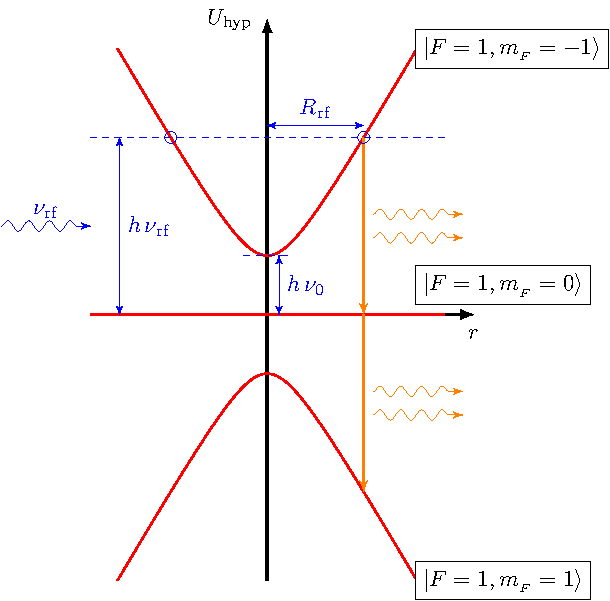
\includegraphics{P1/MesureTempTrans}
\CaptionFig{Représentation schématique des transitions entre \snZs pour des atomes soumis à une onde \rf. La situation considérée ici est celle correspondant au potentiel de piégeage magnétique à symétrie cylindrique décrit dans la \autoref{sec:PiegeageMagnetiqueGuide}.
Les atomes, initialement dans l'état \EtatFmF{1}{-1}, peuvent effectuer une transition stimulée vers un état non-piégé. Ceci ne peut toutefois se produire qu'à la condition de vérifier la relation de résonance $ h\,\nurf = \Uhyp(r) $.
La fréquence $\nurf$ définit ainsi un cylindre de rayon $\Rnurf$. Les atomes qui traversent cette surface durant leur évolution deviennent non-piégés et sont perdus. La \rf correspondant à un cylindre de rayon nul est notée $\nu_0$ sur le schéma.}
\label{fig:MesureTempTrans}
\efig

La fréquence $\nurf$ définit ainsi un cylindre de rayon $\Rnurf$%
\nome{\Rnurf}{Rayon du cylindre de \fisp}%
. Les atomes qui traversent cette surface durant leur évolution deviennent non-piégés et sont perdus. 
La longueur de ce cylindre (suivant l'axe du guide) correspond à la portée $\Lantenne$ %
\nome{\Lantenne}{Portée selon l'axe du \gm de l'antenne de \fisp}%
de l'antenne \rf suivant l'axe du \gm et vaut typiquement \cm{20} dans notre cas (ce point est détaillé dans la \autoref{sec:EvapRf}). 
%
\Resultat{\label{Rq:CritereFiltrage}
Éliminer des atomes du jet par application d'une \rf correspond a un \emph{filtrage spatial sélectif}. 
Le critère permettant de déterminer si un atome va être éliminé ou non du jet est un porte sur la trajectoire de l'atome: 
si celle-ci coupe la surface du cylindre de rayon $\Rnurf$ défini par la \rf $\nurf$, l'atome est éliminé du jet. 
}

\casse

La figure~\nref{fig:TrajGuide} illustre la sélectivité de ce critère par des exemples de trajectoires atomiques dans le plan $(x,y)$.
Notons que le critère de filtrage spatial n'est pas seulement lié à l'énergie mécanique transverse $\Etrans$ de l'atome. Il porte en fait sur le couple $(\Etrans, \Lz)$, où $\Lz$ est le moment cinétique de l'atome autour de l'axe du \gm.
%
\bfigh
\vspace{-.5cm}
\subfloat[]
{\label{TrajGuide_a}
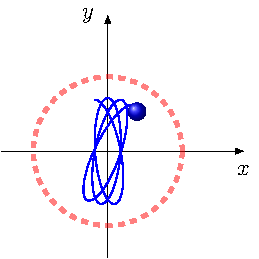
\includegraphics{P1/TrajGuide_a}
}
\subfloat[]
{\label{TrajGuide_c}
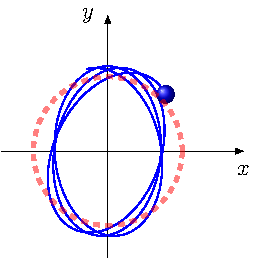
\includegraphics{P1/TrajGuide_c}
}
\subfloat[]
{\label{TrajGuide_b}
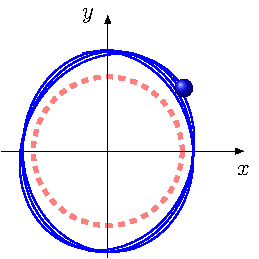
\includegraphics{P1/TrajGuide_b}
}
\CaptionFig{Représentation dans le plan transverse $\xy$ de trajectoires atomiques typiques dans le potentiel de \cthyp $\Uhyp(x,y)$. La présence d'une \rf $\nurf$ définit un cylindre de rayon $r=\Rnurf$. Tout atome traversant la surface de ce cylindre change de \snZ, et est éliminé du jet. La trajectoire (a) correspond à un atome qui ne sera pas éliminé car l'atome n'atteint jamais le rayon $\Rnurf$. L'atome ayant la trajectoire (b) sera éliminé puisque celle-ci coupe le cylindre de filtrage. Notons qu'un atome ayant la trajectoire (c) ne sera pas éliminé malgré le fait que son énergie mécanique est relativement élevée (l'atome orbite en permanence à l'extérieur du cylindre).}
\label{fig:TrajGuide}
\efigh

%\Remarque
{
Dans le cas où le \jat soumis à l'onde \rf est à l'\eqthdy, il est commode d'introduire le \emph{paramètre de filtrage} sans dimension $\eta$ %
\nome{\eta}{Paramètre sans dimension décrivant le \fisp du jet}%
défini comme suit:
\begin{equation}
	\eta
	 \equiv \frac{\Uhyp\left( \larger{\Rnurf}\Rnurf \right) - \Uhyp\left( \larger{\Rnurf} 0 \right) }{\kb\,\Ttrans}
	 = \etaexpr,
	\label{eq:Eta}
\end{equation}
%où $\nu_0$ est la fréquence qui correspond à un filtrage de particule sur un cylindre de rayon nul (par definition, $h\,\nu_0 \equiv \mu\,\Bpara$, voir figure~\nref{fig:MesureTempTrans}).\\
Ce paramètre $\eta$ est défini par le rapport des deux énergies en jeu lors du \firf :
\begin{itemize}
	\item l'énergie potentielle $\Uhyp(\Rnurf)-\Uhyp\left( 0 \right)$ qui correspond à la surface du cylindre de filtrage,
	\item l'énergie thermique transverse moyenne $\kb\,\Ttrans$ des atomes du jet.
\end{itemize} }


		\subsubsection{Exploitation quantitative d'un \spfirf}
		La méthode spectroscopique de détermination de la \tempt repose sur la mesure du \fat après une zone de filtrage sélectif induit par une antenne \rf. 
La figure~\nref{fig:SpectreEvap} donne un exemple de courbe obtenue quand, pour un flux incident $\flux$ donné, on mesure le flux $\fluxapres$ d'atomes qui restent après passage au travers de la zone de \fisp , en fonction de la \rf $\nurf$ utilisée pour effectuer le filtrage. La grandeur pertinente à prendre en compte est en fait le rapport des flux :%
\nome{\rapflux(\nurf)}{Fraction du flux restant après l'action dune zone de \fisp}%
\begin{equation}
	\rapflux(\nurf) \equiv \frac{\left.\fluxapres\right|_{\nurf}}{\flux}
	\label{eq:rapportflux}
\end{equation}
On appellera ce type de courbe expérimentale un \emph{\spfirf}, ou plus simplement, un \termetech{\spfi}. \`A partir de ces données, et en connaissant les caractéristiques du confinement, il est possible de déterminer la \tempt d'un jet supposé à l'\eqthdy.

\pagebreak

\bfighss
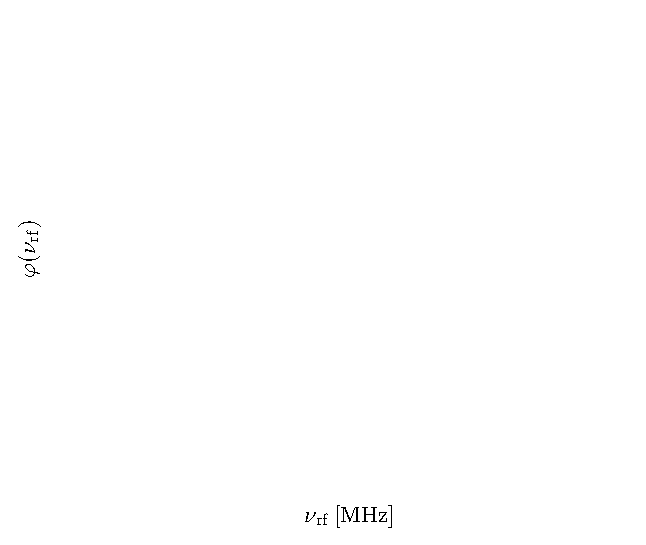
\includegraphics{P1/WithoutEvap}
\CaptionFigsss{Mesure du rapport des \fats avant, et après filtrage spatial du jet en fonction de la \rf $\nurf$ utilisée. Une telle courbe est caractéristique de la distribution transverse $(\Etrans, \Lz)$ d'un \jat à l'\eqthdy. Pour ces données expérimentales, le \ppt est linéaire ($\Bpara=0$), et le \gtchm est $\gradB = \gausspcm{600}$.
}
\label{fig:SpectreEvap}
\efigh

%\Intuition
{
On comprend le comportement asymptotique de la courbe représentée sur la figure~\nref{fig:SpectreEvap}:
\begin{itemize}
	\item pour $\nurf \rightarrow \nu_0$, \cad pour $\eta \rightarrow 0$, le rayon du cylindre de filtrage $\Rnurf$ devient très petit devant l'extension transverse du jet. Les atomes éliminés sont ceux qui passent à proximité immédiate de l'axe du \gm. Le nombre d'atomes concernés est d'autant plus faible que le rayon $\Rnurf$ est petit. Pour un rayon nul, aucun atome n'est élliminé et nous avons donc :
	\[ 
	\rapflux(\eta \rightarrow 0) = 1 
	\pointformule
	\]
	\item pour $\nurf \rightarrow \infty$, \cad pour $\eta \rightarrow \infty$, le cylindre de filtrage contient tous les atomes, et aucun ne traverse sa surface:%. Tous les atomes sont conservés :
	\[ 
	\rapflux(\eta \rightarrow \infty) = 1 
	\pointformule 
	\]
	\item par ailleurs, la largeur de cette courbe est directement liée à la température du jet. En effet, si des atomes sont éliminés sur une large plage de \rf, cela traduit le fait que les atomes \sotosay{explorent} une large plage du potentiel, synonyme d'une température élevée. \`A l'inverse si les atomes sont éliminés sur une petite plage de fréquence, cela traduit le fait qu'il sont confinés tout près de l'axe: la température est faible.
\end{itemize}
}

\casse

Le détail des calculs permettant d'exploiter un \spfirf est donné dans la thèse de T.~Lahaye~\cite{TTL} et nous n'en préciserons ici que les points importants.
Il n'existe pas d'expression analytique%
%
\footnote{Il existe une formule analytique dans le cas $\alpha \gg 1$, \cad quand les atomes \sotosay{voient} un potentiel harmonique \bd. La fraction $\rapflux(\eta)$ d'atomes restant dans le jet est alors donnée par : $ \left. \rapflux(\eta) \right|_{\alpha \ll 1} = 1 - \sqrt{\pi\,\eta}\,\expo{-\eta}$} %
%
 donnant la fraction d'atomes $\rapflux(\eta)$ restant dans le jet en fonction du paramètre $\eta$. 
%
Cependant, moyennant quelques approximations, il est possible d'aboutir à une expression numérique approchée d'interpolation permettant d'exploiter les données expérimentales d'un \spfirf :
\vspace{-1ex}
\inlinefig{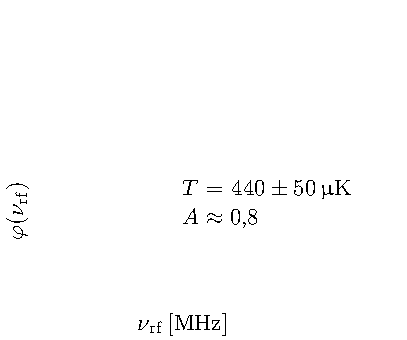
\includegraphics{P1/WithoutEvapFit}}
\begin{equation}
	\rapflux(\eta, \alpha) 
	 = 1 - A\,\left[ \val{1.7}\, \eta^{\val{1.1} - \val{0.4}\,\arctan(\val{3.6}\,\alpha)}
	\,\expo{-\val{0.9}\,\eta} \right] \nonumber
	\virguleformule
\label{eq:FitFunctionRapFlux}
\end{equation}
où la variable $\nurf$ intervient dans la définition de $\eta$, et où le paramètre ajustable $\Ttrans$ apparait dans les expressions de $\eta$ et $\alpha$ (voir les équations~\nref{eq:alpha} et~\nref{eq:Eta}).
$A$ est un paramètre désignant \emph{l'efficacité} de l'antenne \rf utilisée pour effectuer le filtrage. Nous tenons ainsi compte du fait que, sur les atomes devant être éliminés par la zone de \firf, seule une fraction $A$ l'est effectivement.
%Rappelons que cette formule n'est utilisable que si l'on suppose que le \jat est à \eqthdy.
Dans la pratique, nous utilisons cette formule pour ajuster les deux paramètres inconnus $A$ et $\Ttrans$ sur les données expérimentales d'un \spfirf. La figure ci-contre montre les données de la figure~\nref{fig:SpectreEvap} ainsi que la fonction d'ajustement qui permet de déterminer la température du jet. 
L'efficacité d'une antenne est typiquement de $A = \val{80}\%$.

\RemarqueTitre{Précision obtenue grâce à la formule approchée}{
Une série de simulations numériques Monte-Carlo a montré que cette formule approchée permet de déterminer la \tempt du \jat avec une erreur inférieure à $5\%$, et ce, pour une gamme de valeurs de $\alpha$ allant de $\val{0.1}$ à $\val{10}$. 
}

\subsubsection{Mise en \oe uvre expérimentale}
La figure~\nref{fig:MesureTempGuideImplementation} décrit la mise en \oe uvre du protocole de mesure de la \tempt sur le \setup. 
%On y montre aussi une photographie d'une antenne \rf. 
Plus de détails techniques sont fournis dans la thèse de T.~Lahaye~\cite{TTL}.

\bfigh
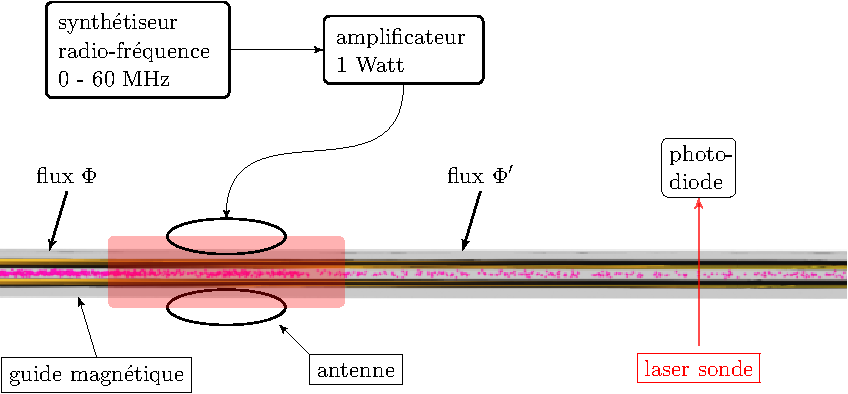
\includegraphics{P1/MesureTempGuideImplementation}
\CaptionFig{Mise en \oe uvre du protocole de mesure de la \tempt. Un synthétiseur  fournit une \rf $\nurf$. Cette onde est alors amplifiée jusqu'à une puissance de l'ordre du Watt. L'antenne disposée sur le \gm permet de diffuser localement l'onde sur les atomes piégés. Il faut noter que la portée de cette antenne au niveau du guide est d'environ \cm{20}(zone grisée sur le schéma). En aval de l'antenne, \cad après le filtrage, nous effectuons une mesure du \fat $\fluxapres$ par la technique décrite dans la \autoref{sec:MesureDensiteGuide}. 
%\\ Comme dit précédemment, la grandeur expérimentalement pertinente est le rapport $\rapflux = \ttfrac{\fluxapres}{\flux}$ des flux avant et après la zone de filtrage. %Le \fat avant filtrage est mesuré tout simplement en stoppant l'émission \rf. 
\\
Notons que le \sotosay{lieu physique} où la \tempt du jet est mesurée est donné par la position de l'antenne \rf, et non par la position du laser sonde. En effet, c'est au niveau de l'antenne que se joue le processus de filtrage qui détermine la fraction $\rapflux$ d'atomes qui atteindra le laser sonde.
}
\label{fig:MesureTempGuideImplementation}
\efigh

		\subsubsection{Limites de la méthode}
	La méthode spectroscopique de détermination de la \tempt par \firf est très fiable. Elle n'est toutefois pas utilisable dans tous les cas de figure. De manière à pouvoir l'appliquer, il faut notamment avoir à l'esprit les deux hypothèses importantes implicitement faites pour mener à bien le calcul de la fraction $\rapflux(\eta)$ d'atomes restant après une zone de \firf:
	\begin{itemize}
	\item les \colels au sein du \jat sont négligées pendant toute la traversée de la zone de \firf,
	\item le rôle de la gravité est négligé.
\end{itemize}	
On comprend bien le rôle de la première hypothèse: si elle n'est pas vérifiée, les collisions vont redistribuer les trajectoires atomiques \emph{pendant le filtrage}. En conséquence, en plus d'éliminer les atomes vérifiant le critère de filtrage, certains atomes \emph{ne vérifiant initialement pas} ce critère, vont pouvoir changer de trajectoire et finalement être aussi éliminés du jet.
\ApplicationNumerique
{Dans le cas de notre \jat, le \tcolel le plus élevé obtenu est $\gammacol \approx \smun{5}$. La portée $\Lantenne$ d'une antenne \rf est typiquement de \cm{20}. En considérant une vitesse du jet typique $\vjet = \cmps{60}$, le nombre de collisions durant la traversée de la zone de filtrage est donc estimé par :
\[
 \frac{\gammacol \, \Lantenne}{\vjet} < 2 \mbox{ collisions}
 \pointformule
 \]
Dans ces conditions, des simulations numériques Monte-Carlo ont montré que cette technique de mesure de température reste très fiable%
\footnotemark.
}
\footnotetext{Avec $\Ncol = 12$, la température est surestimée de près de $20\%$.}
La deuxième hypothèse vise à simplifier la modélisation du problème. La force de gravité rompt la symétrie cylindrique du potentiel de piégeage. Le moment cinétique ne peut donc plus être considéré comme étant une constante du mouvement. De plus, la surface du cylindre de filtrage ne correspond plus à une surface équipotentielle. Cette hypothèse est raisonnable dans le cas de notre configuration expérimentale (on se reportera à la thèse de T. Lahaye~\cite{TTL} pour plus de détails).
\ApplicationNumerique{
Comparons la force de gravité à la force de rappel provenant du \gtchm. Il s'agit donc de comparer $m\,g$ à $\mu\gradB$. Dans le cas du \Rb dans le \snZ $\EtatFmF{1}{-1}$, l'égalité de ces deux forces est obtenue pour un gradient:
\[
\gradB = \frac{m\,g}{\mu} \approx \gausspcm{30}
\pointformule
\]
Or, dans nos expériences, le \gtchm auquel sont soumis les atomes est plus d'un ordre de grandeur supérieur à cette valeur.
}




\section{Évaporation par cycles discrets et gain d'un facteur 10 dans l'\edpup}\label{sec:EvapRf}

Dans la section précédente, nous avons abordé le principe de la mesure de la \tempt du \jat par l'exploitation d'un \spfirf. 
%Fort de connaître la température du jet grâce à cette technique, il est alors 
Dans cette section nous allons montrer qu'il est possible d'utiliser le même principe de \fispse pour éliminer de manière contrôlée certaines classes d'atomes du jet possédant une énergie mécanique transverse élevée afin de modifier les caractéristique du jet. C'est le principe mis en \oe uvre lors du \rpef d'un nuage atomique.% (voir la \autoref{sec:RefEvap}). 

Une étude détaillée de l'\evap du \jat est menée dans le chapitre 4 de la thèse de T. Lahaye~\cite{TTL} et je ne rappellerai donc ici que les résultats et concepts importants que j'ai eus à manipuler lors de mes deux premières années de thèse.

\Resultat{
Afin d'éviter toute confusion, il est important pour la suite de distinguer le \firf utilisé dans les deux cas suivant:
\begin{itemize}
	\item le cas décrit précédemment de la mesure de \tempt qui exploite la mesure expérimentale d'un \spfirf. Cela consiste à \emph{mesurer les caractéristiques} d'un \jat à l'\eqthdy. Cette mesure fait intervenir une antenne utilisée à différentes fréquences $\nurf$, ainsi qu'un laser sonde pour mesurer les variations de flux $\rapflux(\nurf)$.
	\item le cas décrit dans la suite de l'utilisation d'une zone de \firf dans le but précis de \emph{modifier les caractéristiques} du \jat par un processus d'\evap.% (voir la \autoref{sec:EvapForcee}).
\end{itemize}
Dans toute la suite, et sauf mention contraire, le \firf fera référence au deuxième cas.
}


\casse


\subsection{Rethermalisation du jet après une zone de filtrage \rf}\label{sec:RethermJet}
%Jusqu'à présent, nous nous sommes intéressés aux variations de \fat engendrées par 
Le filtrage de certaines classes de trajectoires atomiques au sein du jet est synonyme d'une mise hors d'\eqthdy.	
L'étude de la relaxation de ce jet \sotosay{filtré} vers un nouvel état d'équilibre a été exposé en détail dans les références~\cite{TTL,LaG05}%, et nous n'en rappellerons donc que les résultats importants
.

Les prédictions théoriques obtenues reposent simplement sur un bilan d'énergie et de nombre de particules. 
%\Resultat
{
Les caractéristiques du jet à l'\eqthdy avant le filtrage étant données par les cinq paramètres $(\vjet, \flux, T, \gradB, \alpha)$ et l'énergie mécanique moyenne d'une particule étant notée $\Emoy$, le bilan est effectué entre deux instants:
\begin{itemizel}
	\item tout de suite après le filtrage spatial du jet, le flux de particules $\fluxapres$ ainsi que l'énergie moyenne $\Emoyapres$, sont déduits de la manière décrite dans la \autoref{sec:MesureTempTrans},
	\item un temps arbitrairement long après le filtrage, le jet étant supposé avoir atteint son nouvel état d'\eqthdy défini par $(\vjet, \fluxapres, T', \gradB, \alpha')$.
\end{itemizel} 
La conservation de l'énergie et du nombre de particules pendant le processus de retour vers un nouvel état d'\eqthdy (grâce aux \colels) permet alors de déduire la nouvelle température $T'$ du \jat.
}

Il n'existe pas de formulation analytique donnant $T'$ en fonction du paramètre de filtrage $\eta$ dans le cas d'un \cthyp%
%
%\footnote{Comme dans la section~\nref{sec:MesureTempTrans}, il existe une formule analytique dans le cas $\alpha \ll 1$, \cad quand les atomes sont confinés dans un potentiel harmonique bi-dimensionnel. Pour plus de détails, on se reportera à la référence~\cite{TTL}%. La nouvelle température  d'\eqthdy est alors donnée par \[ \left. \frac{T'}{T} \right|_{\alpha \ll 1} = 1 - \sqrt{\pi\,\eta}\,\Expo{-\eta}\].}%
.
\ifthenelse{\FormatEUE > 0}{}
{\AjouteLigne}
En pratique, une intégration numérique est utilisée pour pouvoir prédire le comportement du \jat. Nous montrons dans la figure~\nref{fig:TsurTGuide} la courbe donnant la variation de température $\tfrac{T'}{T}$ en fonction du paramètre de filtrage $\eta$ dans les deux cas asymptotiques $\alpha \gg 1$ (correspondant à un \pthar) et $\alpha \ll 1$ (correspondant à un \ptlin).
\bfighs
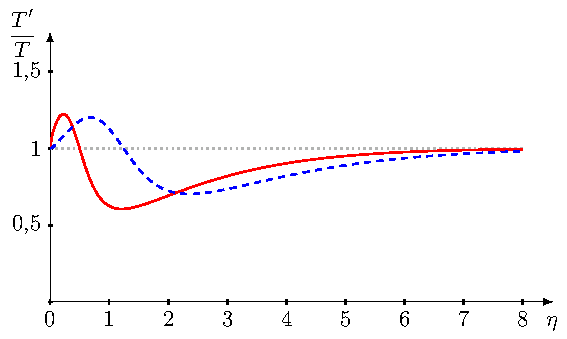
\includegraphics{P1/TsurTGuide}
\RemonteUnPeuFig\RemonteUnPeuFig
\CaptionTocCaptionFig{Variations relatives de la température du jet après une zone de \firf}{Variations relatives $\ttfrac{T'}{T}$ de la température du jet après une zone de \firf de paramètre $\eta$, et une \reth complète. La courbe est représentée dans les deux cas limites d'un \cthar, $\alpha \gg 1$ (trait plein), et d'un \ctlin $\alpha \ll 1$ (trait tireté). Il est possible de refroidir le \jat si $\eta$ est supérieur à une valeur limite $\etalim$. Le comportement asymptotique de ces courbes est bien compris:\\
\vtop{\linewidth=\CaptionWidth %
\begin{itemize}
\item pour $\eta \gg \etalim$, les atomes éliminés du jet possèdent une grande énergie mécanique, supérieure à l'énergie moyenne $\Emoy$. L'énergie moyenne par atome $\Emoyapres$ après le filtrage est donc plus faible. La nouvelle température d'équilibre est plus faible,  $\ttfrac{T'}{T} \lesssim 1$.
\item pour $\eta \ll \etalim$ les atomes éliminés possèdent globalement une énergie mécanique inférieure à l'énergie moyenne. L'énergie moyenne par atome augmente donc. La nouvelle température d'équilibre est plus élevée, $\ttfrac{T'}{T} \gtrsim 1$.
\item par ailleurs, si le rayon du cylindre de filtrage est nul ($\eta \rightarrow 0$), ou infini ($\eta \rightarrow \infty$), aucun atome n'est éliminé, et la température reste inchangée, $\ttfrac{T'}{T} = 1$.
\end{itemize}
}
}
\label{fig:TsurTGuide}
\efigh

\pagebreak

\noindent
Sur la figure~\nref{fig:TsurTGuide}, on constate qu'il est possible de refroidir le jet si $\eta$ est pris suffisamment grand: 
\begin{itemizel}
	\item $\eta > \val{0.5}$ pour un piégeage transverse harmonique.
	\item $\eta > \val{1.18}$ pour un piégeage transverse linéaire.
\end{itemizel}

\EnFaitNon{\nRemarque{Le fait qu'il soit aussi possible de chauffer le jet peut paraître surprenant de prime abord \dixit{si l'on se représente, à tort, le processus d'\evap comme l'élimination des particules les plus énergétiques. En effet, nous avons vu page \pageref{Rq:CritereFiltrage} que le critère de filtrage porte non pas sur l'énergie d'un atome, mais sur le couple (énergie, moment cinétique). La figure \vref{fig:TrajGuide} montre d'ailleurs que certains atomes très énergétiques sont conservé lors de la phase de filtrage.}
}
}

\noindent \dixit{Nous devons maintenant nous demander comment varient les deux paramètres cruciaux du jet:
\begin{itemizel}
	\item la \ddedpup $\rhojetaxe$ sur l'axe $z$,% que l'on veut augmenter le plus possible, 
	\item le \tcolel $\gammacol$.% qui doit rester important, voire augmenter. C'est en effet ce paramètre qui détermine la cinétique du retour à l'équilibre\footnote{Si $\gammacol$ devient très faible, cela veut tout simplement dire que le refroidissement (au sens d'atteindre un nouvel état d'\eqthdy) ne se fait qu'au bout d'un temps extrêmement long.}.
\end{itemizel}
}

La figure \vref{fig:RhoGammaGuide} représente les variations attendues $\ttfrac{\rhojetaxeapres}{\rhojetaxe}$ et $\ttfrac{\gammacolapres}{\gammacol}$ de ces deux grandeurs, dans les deux cas limites $\alpha \gg 1$ et $\alpha \ll 1$.
\bfigsss
\subfloat[]{\label{fig:RhosurRhoGuide}
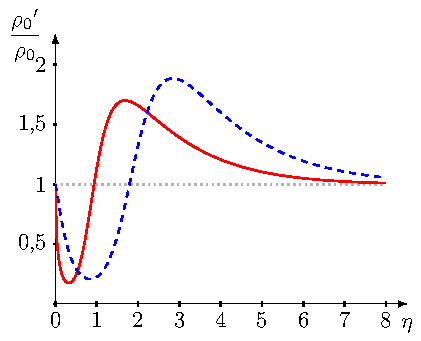
\includegraphics{P1/RhosurRhoGuide}}
\subfloat[]{\label{fig:GammasurGammaGuide}
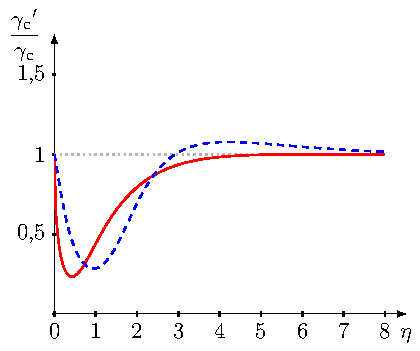
\includegraphics{P1/GammasurGammaGuide}}
\CaptionFigs{Courbes représentant les variations relatives (a) de la \ddedpup $\ttfrac{\rhojetaxeapres}{\rhojetaxe}$ sur l'axe $z$ ; (b) du \tcolel $\ttfrac{\gammacolapres}{\gammacol}$ \emph{après une zone de \firf} de paramètre $\eta$, et une \reth complète. Sont envisagés ici les deux cas limites d'un \cthar, $\alpha \gg 1$ (trait plein), et d'un \ctlin $\alpha \ll 1$ (trait tireté).
}
\label{fig:RhoGammaGuide}
\efig

\noindent Cette figure montre notamment que la \ddedpup augmente si $\eta$ est choisi suffisamment grand. En revanche, on constate que le \tcolel ne peux pas être augmenté dans le cas d'un \cthar%
%
\footnote{En toute rigueur, il est théoriquement possible dans un \cthar et pour $\eta \approx 7$, d'augmenter le \tcolel d'environ $\val{0.1}\%$. Ce qui n'est en pratique absolument pas exploitable.}%
. 
Le \ctlin semble être plus profitable du point de vue du processus d'\evap. En effet: 
\begin{itemize}
	\item  le gain relatif en \ddedpup peut alors atteindre $\val{1.9}$ contre $\val{1.7}$ pour un piégeage harmonique,
	\item ce gain maximum est obtenu pour un paramètre $\eta \approx \val{2.9}$ qui, sur le plan du \tcolel, correspond à une augmentation sensible de quelques pour cent. Le piégeage harmonique implique une diminution d'environ $25\%$ du \tcolel si l'on désire obtenir le gain maximal de $\val{1.7}$ en \ddedp%
	%
\footnote{Dans ces conditions, l'enchainement de 5 zones d'évaporation conduirait théoriquement à une réduction du \tcolel par facteur \val{1000}.}.
\end{itemize}

\Remarque{
L'impossibilité d'augmenter le \tcolel $\gammacol$ dans le cas du potentiel harmonique est propre au caractère \bd du confinement~\cite{LaG06,DMK95}. 
Il est tout à fait possible d'augmenter le $\gammacol$ dans un piège harmonique \td (tel qu'un piège de \IP). 
Cette limite est un lourd handicap puisqu'elle interdit l'\termetech{emballement} du processus d'évaporation%
%\footnote{L'\termetech{emballement} traduit l'augmentation du \tcolel au fur et à mesure de l'évaporation, qui permet}%
.
% telle qu'elle est décrite dans la \autoref{sec:EvapForcee}. 

L'utilisation d'un potentiel \tlin ($\alpha \ll 1$) semble donc souhaitable. Cependant, le paramètre $\alpha$ est déterminé par la température du jet. En atteignant des températures de plus en plus faibles, on finira toujours par avoir $\alpha > 1$.
}


\RemonteUnPeuFig
\RemonteUnPeuFig

\subsection{Gain d'un facteur 10 dans l'\edpup}\label{sec:Gain10}
\noindent \dixit{Dans la sous-section précédente, la dynamique du retour à l'\eqthdy via les \colels entre atomes a été complètement passée sous silence. Or, il s'agit d'un point crucial dans la perspective d'un refroidissement poussé du jet.
} 
Le temps nécessaire au jet pour effectuer son retour à un \eqthdy se formule en termes de nombre moyen $\Ncol$ de \colels entre atomes. Pour plus d'information, on consultera avec intérêt les références~\cite{LaG05,LaG06}%
%
\footnote{Un point remarquable est détaillé ces deux articles. Celui-ci a initialement été mis en évidence dans la référence~\cite{AnG06}: la dynamique du retour à l'\eqthdy dépend de manière notable de la géométrie du potentiel. Ainsi, dans un \pptlin, un jet mis hors d'équilibre par une zone de \firf va demander, pour \rether, jusqu'à $2$ fois plus de \colels que dans le cas d'un \cthar.}. 

%Nous avons mentionné précédemment qu'u
Une manière d'augmenter le nombre de \colels au sein du \jat est de mettre en place une \secpent dans le \gm. Sur notre \setup, on atteint grâce à ce procédé $\Ncol = 20$. 
\dixit{L'utilisation de plusieurs zones d'évaporation est alors envisageable, dans le but d'obtenir un gain significatif en \ddedp.} 

%\ifthenelse{\FormatEUE > 0}{}
{\AjouteLigne}

\RemonteUnPeuFig
\RemonteUnPeuFig

\subsubsection{Dispositif à 11 zones d'évaporation}
\noindent Sur notre \setup, 11 zones d'évaporation ont été placées le long du \gm (voir la figure~\nref{fig:Montage10Antennes}). 
Elles sont réparties tout les \cm{20}, sauf sur la section centrale où les éléments de connexion en acier empêchent les ondes \rf d'atteindre le jet.
%
\RemonteUnPeuFig
\RemonteUnPeuFig
\bfighss
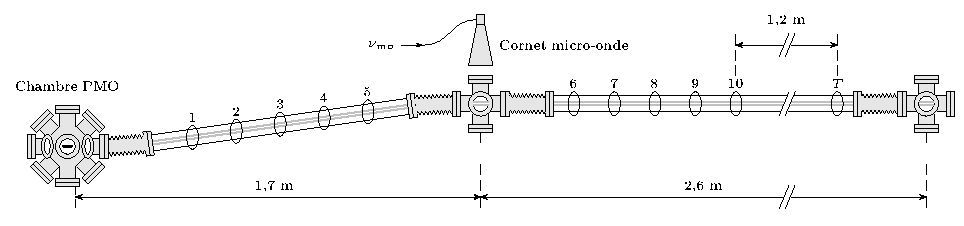
\includegraphics[width=\FigWidth]{P1/Montage10Antennes}
\CaptionFigssss{Disposition des antennes \rf (représentées par des ellipses numérotées de 1 à 10) et du cornet micro-onde utilisés pour produire l'enchainement de zones d'évaporation du \jat.
Des connexions en acier permettent de joindre les deux sections du tube de verre entourant le guide. Seules les micro-ondes permettent une évaporation efficace du jet dans cette zone. 
Notons qu'une distance de \m{1.2} à la fin du guide est dépourvue de zone d'évaporation afin de permettre le retour à l'\eqthdy du jet avant d'effectuer la mesure du \spfi qui détermine la température (antenne notée $T$).
}
\label{fig:Montage10Antennes}
\efigh
%

\casse

\nRemarqueTitre{Utilisation d'une antenne micro-onde}{
	Nous avons mis en \oe uvre une technique d'évaporation \emph{micro-onde} sur notre \setup. Celle-ci repose sur le \fisp identique à celui décrit dans la \autoref{sec:RethermJet}, mais en utilisant des transitions entre \snhfs.
Pour plus de détails, on pourra se reporter à la thèse de T.~Lahaye~\cite{TTL}. Mentionnons toutefois les deux avantages de cette technique :
\begin{itemize}
	\item trois transitions, $\EtatFmF{1}{-1}\longrightarrow\EtatFmF{2}{0,1,2}$, sont autorisées. Chacune d'elle correspond, pour une fréquence $\numo$ donnée, à trois rayons de cylindre de filtrage différents. L'évaporation en est rendue plus efficace.
	\item les micro-ondes (à la différence des ondes \rf) se propagent bien à l'intérieur des tubes de connexion en acier qui compose le système à \uv. On peut donc utiliser cette technique pour effectuer l'évaporation à l'intérieur d'une chambre à vide métallique en plaçant le cornet émetteur devant un hublot. Dans le cas plus spécifique du \jatgm, nous pouvons créer une zone de filtrage entre les deux sections du guide (voir la figure~\nref{fig:Montage10Antennes}).
\end{itemize}
}

\ifthenelse{\FormatEUE > 0}{}
{\AjouteLigne}
	
	\subsubsection{Gain en \ddedp}
La figure~\nref{fig:Gain10Spectre} montre les \spfirfs mesurés grâce à la dernière antenne (notée $T$ sur la figure~\nref{fig:Montage10Antennes})  dans les deux cas suivant:
\begin{itemize}
	\item le \jat non refroidi, \cad sans les antennes d'évaporation,
	\item le même jet, mais après son passage dans la succession des 11 zones d'évaporation.
\end{itemize}
%
\bfighs
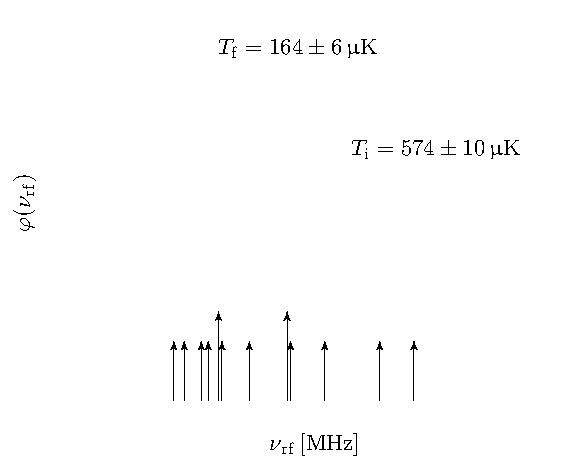
\includegraphics{P1/Gain10Spectre}
\CaptionFigss{Spectre de \firf permettant de déterminer les caractéristiques du \jatgm dans les deux cas du jet non-refroidi (\cad sans les antennes d'évaporation représentées sur la figure~\nref{fig:Montage10Antennes}) et du même jet mais ayant traversé les 11 zones d'évaporation. Les flèches représentent les \rfs utilisées par les antennes. 
Les flèches plus longues correspondent à la zone d'évaporation micro-onde, en termes de \rfs qui donneraient les même rayons d'évaporation.\newline
Le \spfirf initial correspond à une température $\Tini = \microKpm{574}{10}$. Après retour à l'\eqthdy le \spfi est beaucoup moins large, traduisant le fait que la température est plus faible: $\Tfin = \microKpm{164}{6}$}
\label{fig:Gain10Spectre}
\efigh
\Cahier{6,166}

\Resultat%
{
\noindent
Les données expérimentales représentées sur la figure~\nref{fig:Gain10Spectre}, ainsi qu'une mesure du \fat permettent d'effectuer le bilan dans l'encadré ci-dessous:
\vspace{1ex}
\begin{center}
%\begin{Large}
\begin{tabular}{|lcccl|}
\hline
  Jet non évaporé   &    & &  &  Jet évaporé   %\vspace{3ex} 
\\
$\vjet = \cmps{60}$  &    &  &  &  $\vjet = \cmps{60}$    %\vspace{1.5ex}
\\
$\flux \approx \atps{7E{9}}$ &  &\huge{${\Longrightarrow}$} & & $\fluxapres \approx \atps{9E{8}}$     %\vspace{1.5ex}
\\
$T = \microKpm{574}{10}$ & & & & $T' = \microKpm{164}{6}$   \vspace{-2.5ex} %\vspace{1.5ex}
\\
$\underbrace{\phantom{T = \microKpm{574}{10}}}_{}$  &  &  &    & $\underbrace{\phantom{T' = \microKpm{164}{6}}}_{}$  \vspace{-1ex}
\\
$\rhojetaxe \approx \val{2.0E{-8}}$ & & & & $\rhojetaxe \approx\val{2.1E{-7}}$\\ %\vspace{1.5ex}
\hline
\end{tabular}	
%\end{Large}
\end{center}
\vspace{1ex}
Nous démontrons ainsi un gain en \ddedpup d'un facteur $\val{10.4}^\val{+4.1}_\val{-3.0}$. 
%Ce résultat fait l'objet de la référence~\cite{LWR05}. 
}

\section{Conclusion}
	\subsection{Difficultés inhérentes à l'\evap d'un \jatg}\label{sec:DifficultesInherentes}
On peut s'interroger sur le fait qu'il semble difficile d'obtenir un gain sur $\rhojetaxe$ supérieur à 1 ordre de grandeur. En effet l'utilisation du \rpef sur une expérience typique de \condbe permet de gagner plusieurs ordres de grandeur en \ddedpup.

Notons tout d'abord que la succession des 11 zones d'évaporation dont il est question plus haut conduirait théoriquement à un gain \val{1600} sur $\rhojetaxe$, si l'on supposait une \reth complète du jet entre chaque zone. En réalité, le nombre $\Ncol \approx 20$ de \colels au sein du jet ne permet pas d'obtenir ce gain. 

\Resultat
{\label{JetAtomiqueDifficultees}
Soulignons les trois raisons principales qui font que l'\evap d'un \jat est une tâche fondamentalement plus ardue que pour un nuage d'atomes piégés:

\begin{itemize}
	\item le simple fait de produire un \j à partir de l'injection pulsée de \pats implique une \emph{dilution spatiale} des \ps suivant l'axe du \gm. Ceci se traduit par une perte en \dat, et donc en \tcolel%
%	\footnotemark.
	\item le guide ayant une longueur finie, le temps alloué pour réaliser l'évaporation est limité par le \emph{temps de propagation}. En pratique nous disposons d'environ \seconde{6}.
	\item le \emph{confinement purement transverse} rend le processus d'évaporation moins efficace que dans le cas d'un piégeage \td%
	\footnotemark.
\end{itemize}
}
%\footnotetext{La perte en \tcolel dû à la dilution spatiale des \ps est estimée à un facteur $6$.}
\footnotetext{Comme nous l'avons souligné, il est en particulier impossible d'observer un emballement de l'évaporation dans un \ppthar.}

\subsection{Nécessité de développer de nouveaux outils}

Dans ce chapitre nous avons décrit le \setup qui nous a permis de mettre en \oe uvre le \rpef d'un \jatuf \mg. Le gain d'un facteur $10$ sur la \ddedp semble faible face aux sept ordres de grandeur qui nous séparent encore de la \condbe. Le paramètre physique qui nous limite est en fait le nombre moyen $\Ncol$ de collisions subies par un atome au cours de sa propagation. Une estimation montre que si nous pouvions disposer d'un nombre dix fois plus élevé de collisions (soit $\Ncol\approx200$), le \rdq serait alors accessible. La figure~\nref{fig:EvolutionNC} montre l'évolution du nombre de collisions $\Ncol$ lors des différentes évolutions du \setup.
\bfig
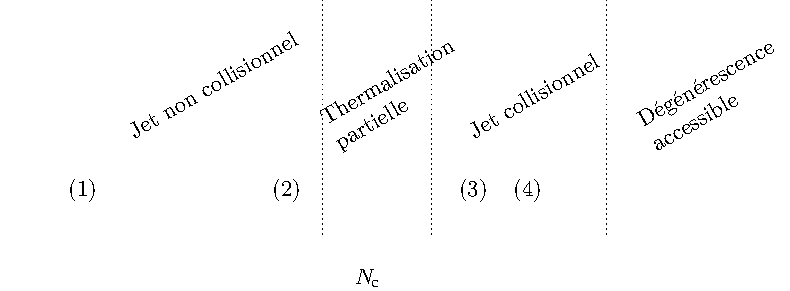
\includegraphics{P1/EvolutionNC}
\CaptionFig{Représentation de l'évolution du nombre de \colels $\Ncol$ subies en moyenne par chaque atome au cours de sa propagation le long du \gm. Les différentes étapes chronologique, dans le cadre de notre expérience, sont représentée par des points: (1) en 2002~\cite{CRA02}, (2) en 2003~\cite{RCL03}, (3) en 2004~\cite{LVG04}, (4) en 2005~\cite{LWR05}.
}
\label{fig:EvolutionNC}
\efig

\noindent La plupart des chapitres de ce manuscrit de thèse sont dédiés à l'étude de différentes possibilités visant à contrecarrer les trois difficultés mentionnées dans l'encadré \vpageref[ci-dessus ][de la ]{sec:DifficultesInherentes} :
\begin{itemize}
	\item le chapitre~\nref{chap:MiroirMobile} présente une nouvelle méthode de ralentissement des \ps injectés dans le guide grâce à l'utilisation d'un \mimamo. Nous montrerons en particulier que cette méthode, contrairement à l'utilisation d'une \secpent, peut théoriquement \emph{augmenter} la \ddedpup du jet obtenu par recouvrement des \ps.
	\item le chapitre~\nref{chap:Convoyeur} traite du transport des \pats dans un train de pièges de Ioffe-Pritchard. Le fait de préserver momentanément (sur le premier mètre du guide) un piégeage \td permet de conserver un \tcolel élevé et de rendre l'évaporation plus efficace.
	\item le chapitre~\nref{chap:PiegeDipolaire} consiste en l'étude de la production de \ps très denses dans un piège dipolaire. En augmentant le \tcolel ainsi que la \ddedp des \pats, nous pouvons espérer produire un \jatuf dont les caractéristiques initiales seraient plus favorables pour mener à bien le \rpef.
\end{itemize}
